% Methods: Income (DL) and EA end — paste into paper.tex or % Methods: Income (DL) and EA end — paste into paper.tex or % Methods: Income (DL) and EA end — paste into paper.tex or % Methods: Income (DL) and EA end — paste into paper.tex or \input{methods_03_04}
% Requires: \usepackage{amsmath,amssymb}

\subsection{Unemployment and SNAP participation (distributed lag)}
\label{sec:income-dl}

We estimate the dynamic response of SNAP participation to \emph{changes} in local unemployment using a distributed-lag (DL) specification in county--month panel data. The regressor is the 12-month change in the unemployment rate, $\Delta u_{ct} = u_{ct} - u_{c,t-12}$, so that coefficients are interpretable as the impulse response to an unemployment shock.

For county $c$ and month $t$,
\begin{equation}
Y_{ct} = \alpha_c + \gamma_t + \sum_{\ell=0}^{L} \beta_\ell \, \Delta u_{c,t-\ell} + \varepsilon_{ct},
\end{equation}
where $Y_{ct} = \ln(1 + \text{recipients}_{ct})$; $\alpha_c$ and $\gamma_t$ are county and month fixed effects; and $L=6$. Standard errors are clustered at the county level. The cumulative effect of a one percentage-point increase in the unemployment rate is $\sum_{\ell=0}^{L} \beta_\ell$.

Heterogeneity is based on \emph{pre-determined} exposure: we split counties by their average unemployment rate over 2014--2016 (before the main ABAWD rollout). The same DL model is estimated separately in the high- and low-exposure subsamples.

% --- Uncomment and adjust figure/table numbers when you add the actual floats ---
% \begin{figure}[htbp]
%   \centering
%   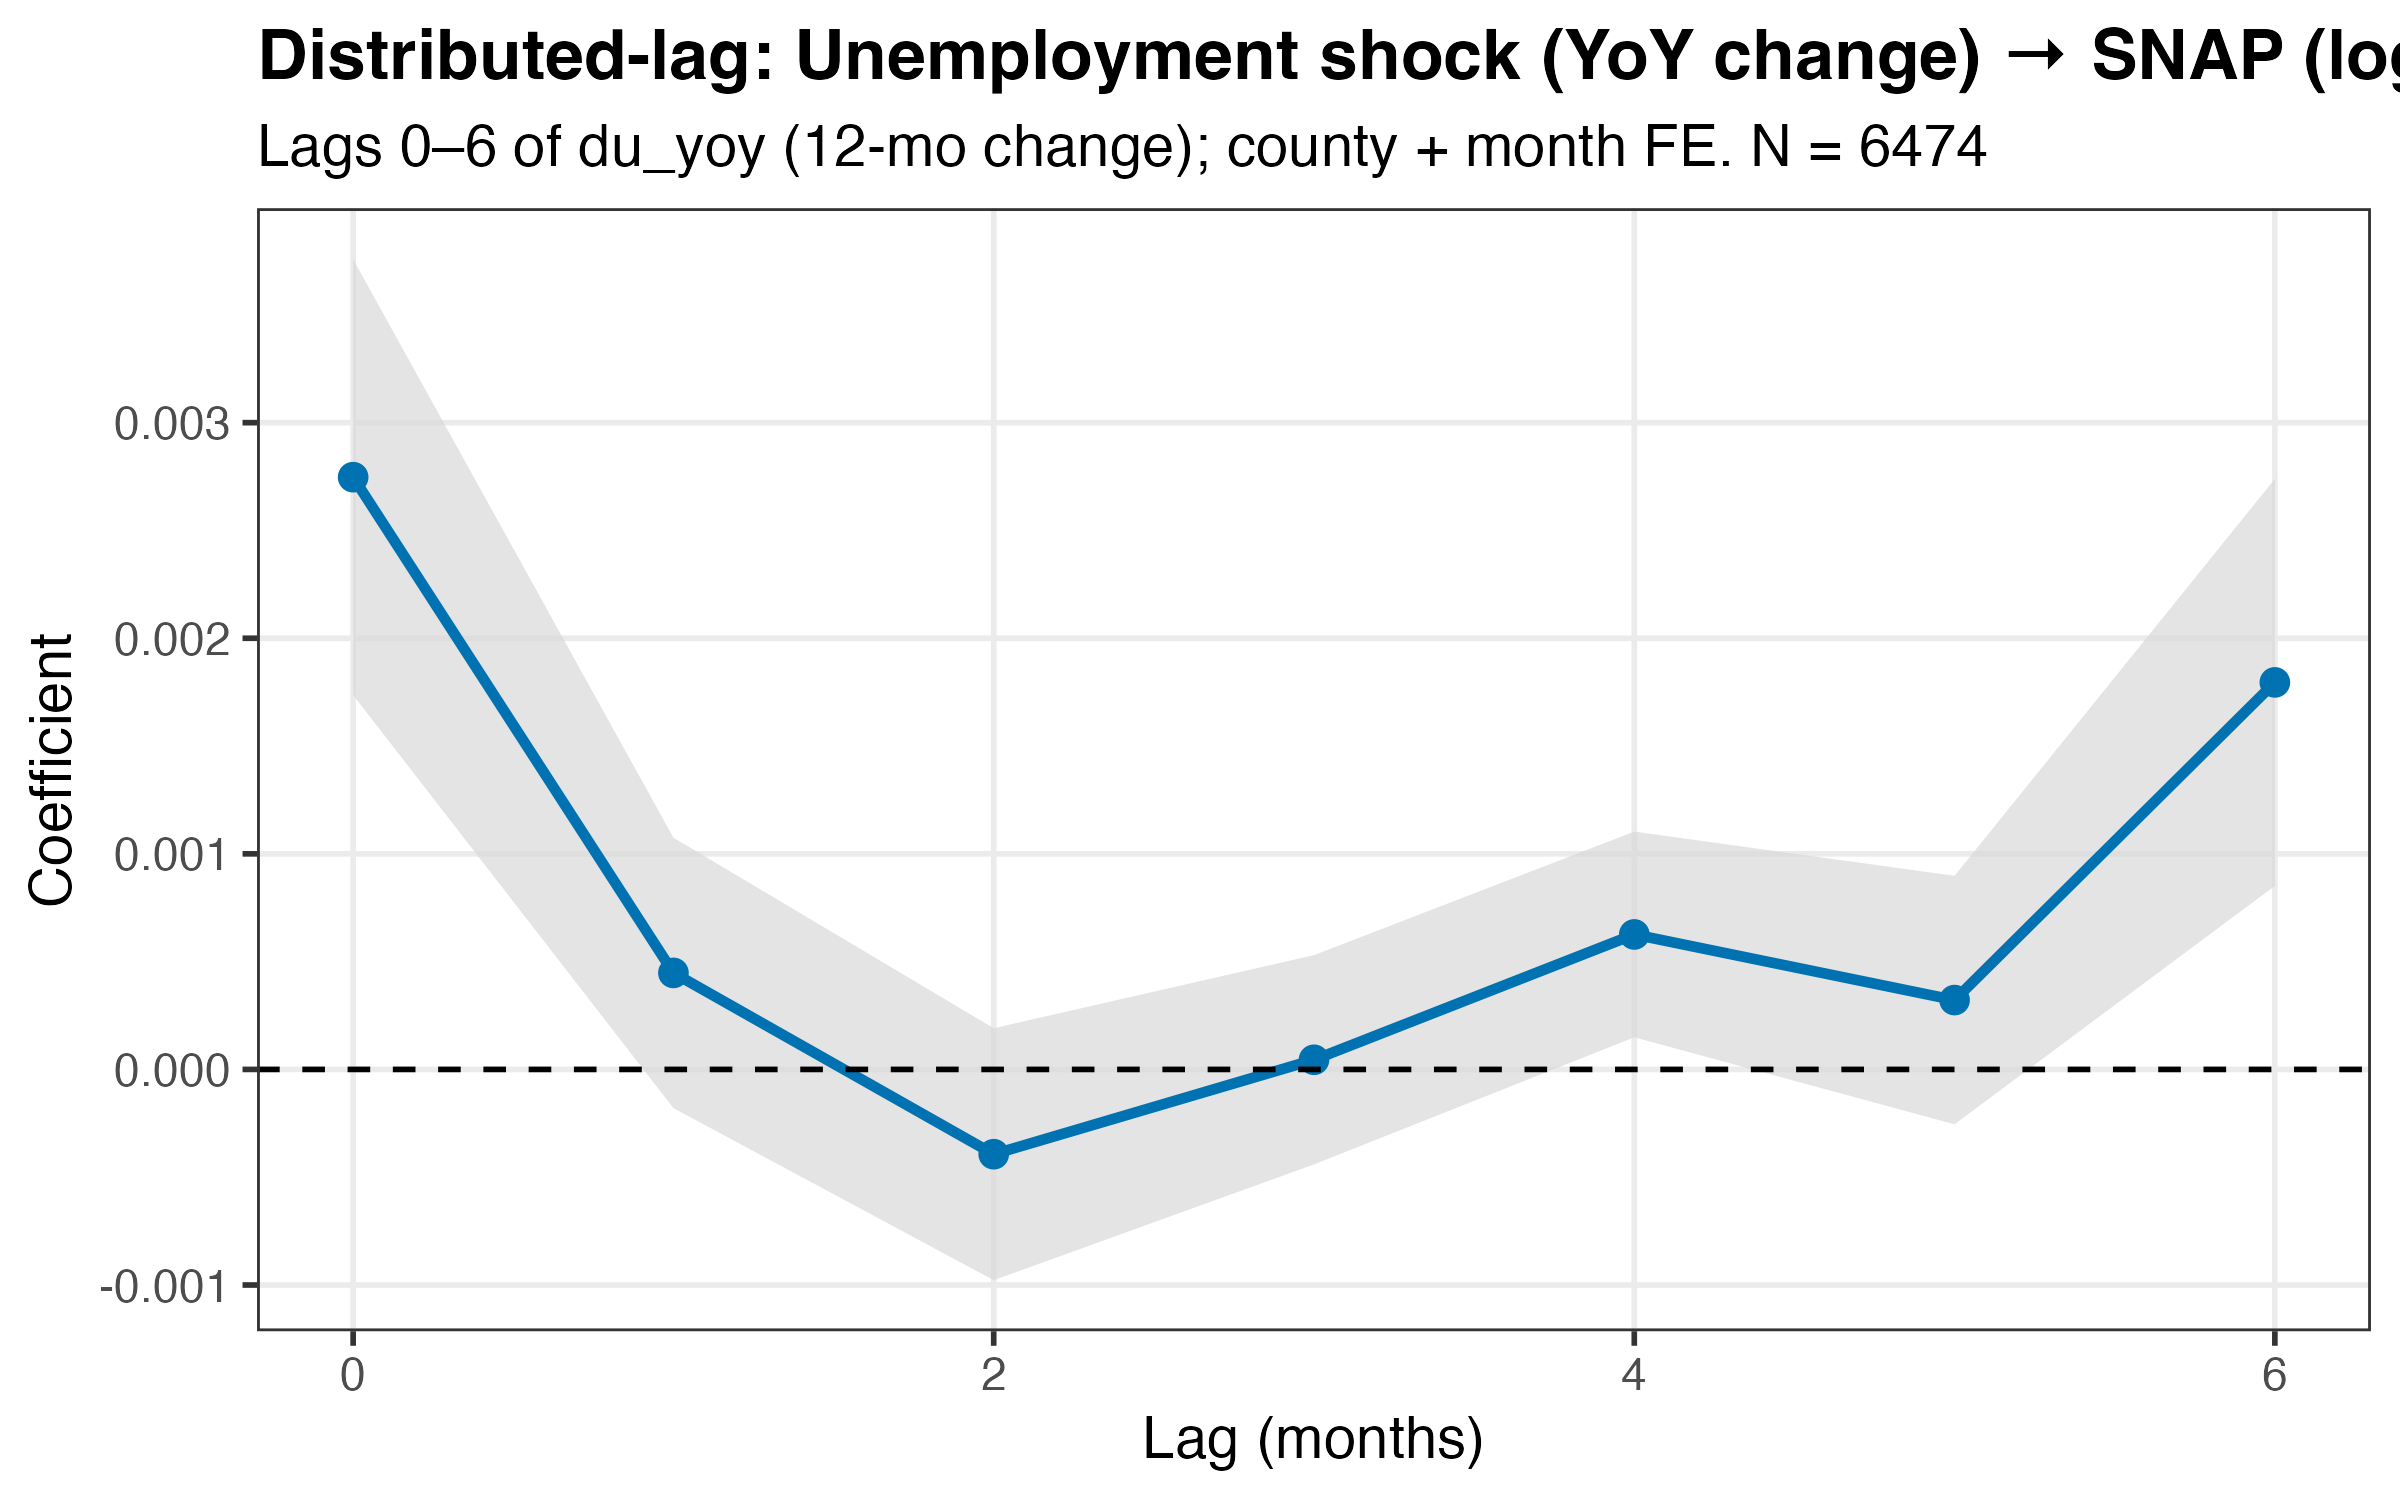
\includegraphics[width=0.85\textwidth]{../outputs/figures/income_dl_recipients}
%   \caption{Distributed-lag: dynamic response of SNAP participation (log 1+ recipients) to 12-month change in unemployment rate. County and month FE; lags 0--6; 95\% CI; SE clustered by county.}
%   \label{fig:income-dl}
% \end{figure}

% \begin{table}[htbp]
%   \centering
%   \caption{Distributed-lag estimates (income DL). Cumulative effect $\sum \beta$ reported in heterogeneity table.}
%   \label{tab:income-dl}
%   \input{../outputs/tables/income_dl_main}  % or manually type key rows
% \end{table}

% ---------------------------------------------------------------------------
\subsection{End of Emergency Allotments (EA) event study}
\label{sec:ea}

Event time is defined in integer months relative to the EA end (March 2023):
\begin{equation}
\text{event time}_t = (12 \times \text{year}_t + \text{month}_t) - (12 \times \text{year}_{\text{EA}} + \text{month}_{\text{EA}}).
\end{equation}

\paragraph{Average benefit (descriptive).}
We estimate $Y_{ct} = \alpha_c + \sum_{k \neq -1} \delta_k \,\mathbf{1}(\text{event time}_t = k) + \varepsilon_{ct}$ for average benefit per person, with $k=-1$ as reference. This documents the drop in benefits at the EA end.

% \begin{figure}[htbp]
%   \centering
%   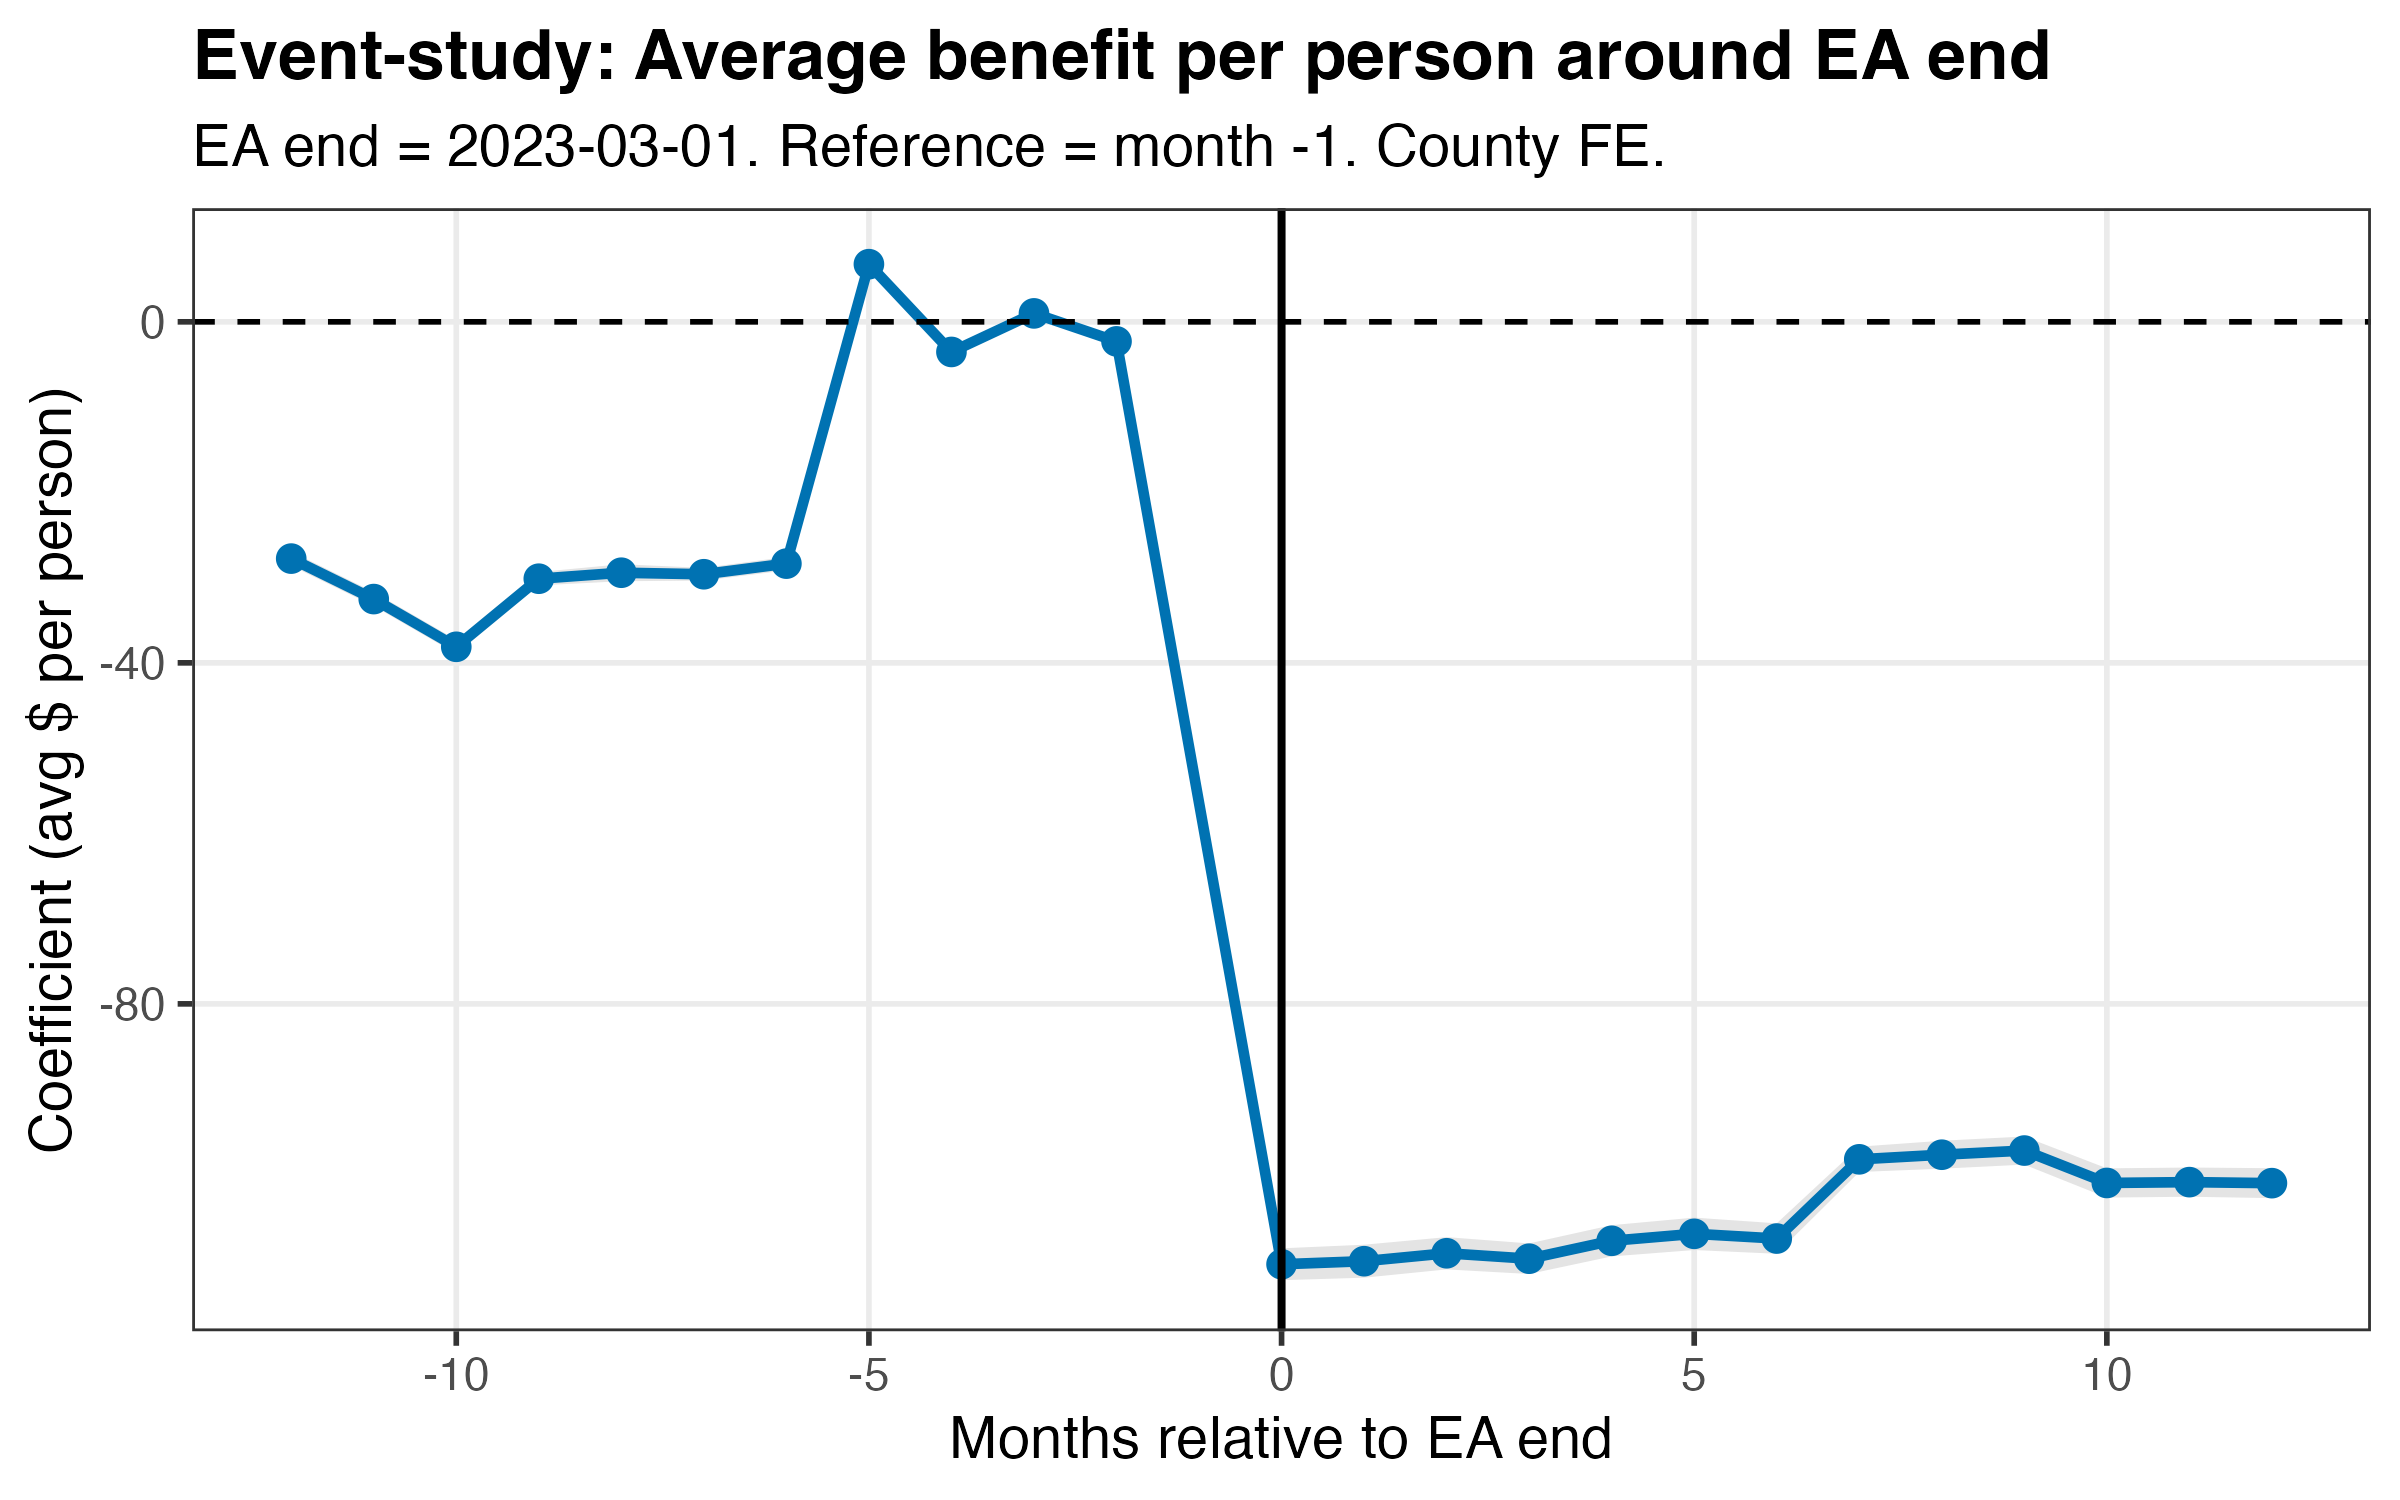
\includegraphics[width=0.85\textwidth]{../outputs/figures/ea_es_avgpp}
%   \caption{Event-study: average benefit per person around EA end. Reference month $-1$; county FE; 95\% CI.}
%   \label{fig:ea-avgpp}
% \end{figure}

\paragraph{Participation: intensity differential (main).}
For participation, we use a differential event-study with month fixed effects. Counties are classified as high or low ``intensity'' by whether their pre-EA (months $-12$ to $-1$) average benefit per person is above the median. We estimate
\begin{equation}
Y_{ct} = \alpha_c + \gamma_t + \sum_{k \neq -1} \theta_k \,\big(\mathbf{1}(\text{event time}_t = k) \times \text{High intensity}_c\big) + \varepsilon_{ct},
\end{equation}
where $\gamma_t$ are month fixed effects. Only the interaction terms are included; $\theta_k$ is the high-minus-low difference at event month $k$ (relative to $-1$), identifying the differential response under common time shocks.

% \begin{figure}[htbp]
%   \centering
%   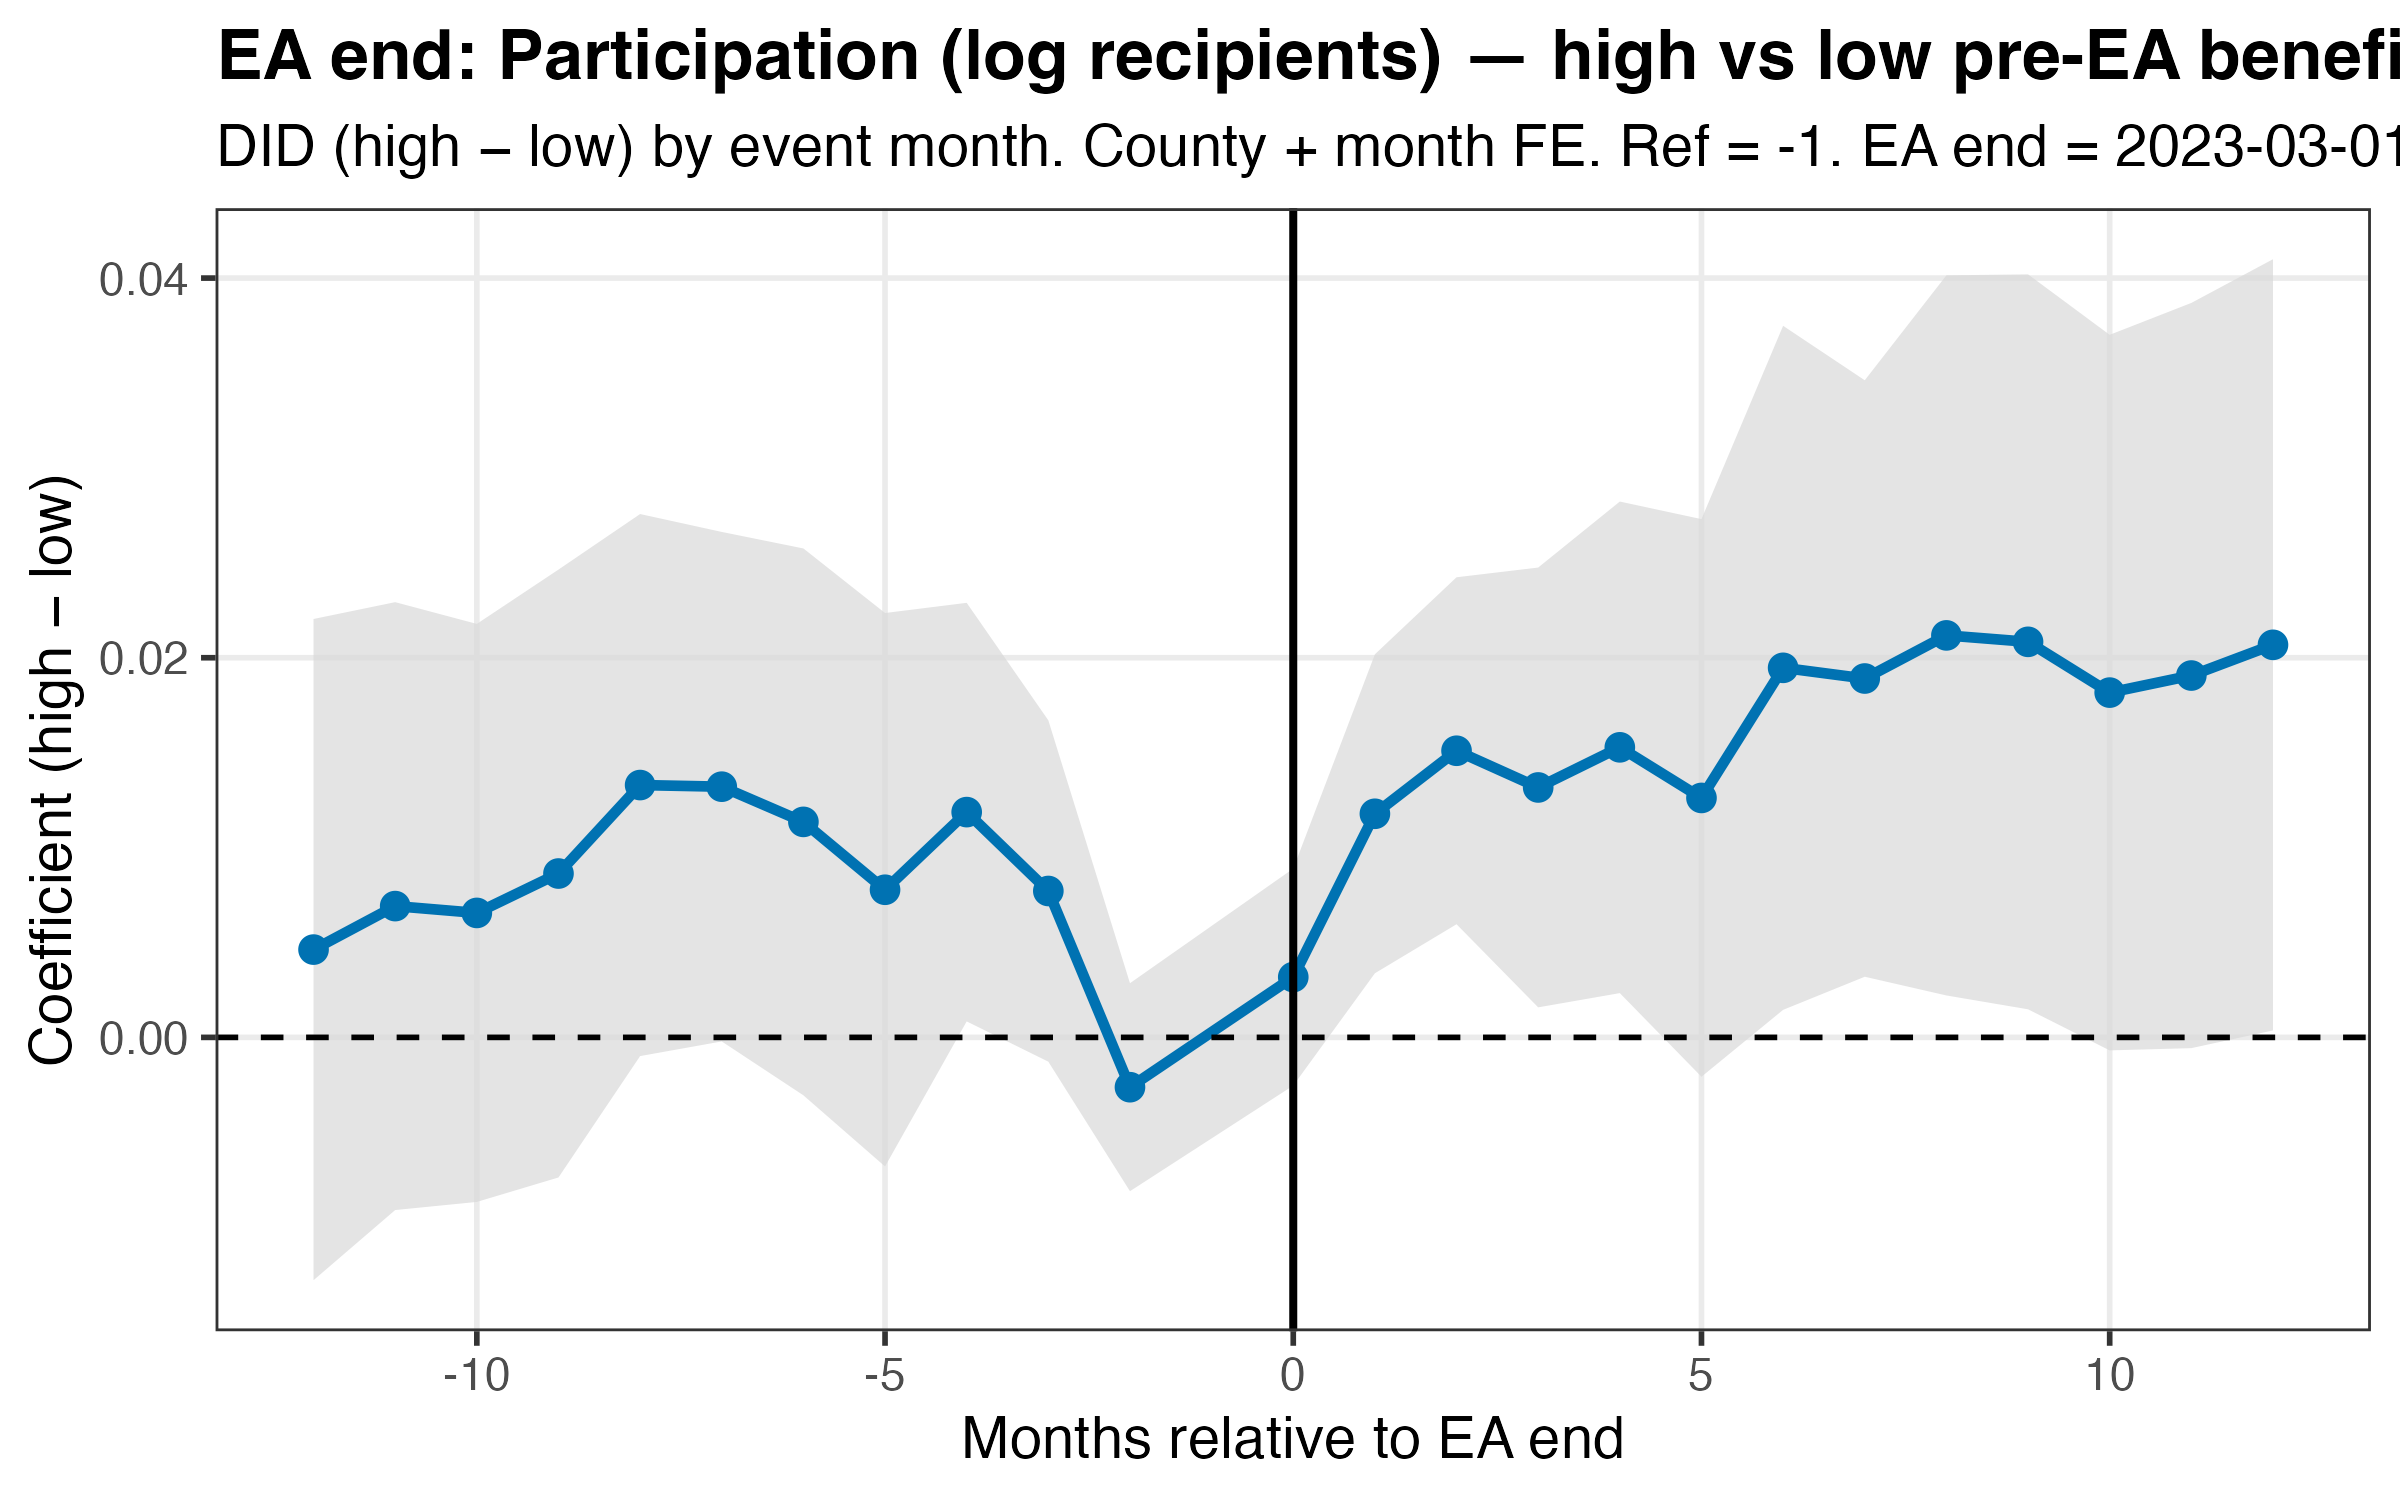
\includegraphics[width=0.85\textwidth]{../outputs/figures/ea_es_participation}
%   \caption{EA end: participation (log recipients), high vs.\ low pre-EA benefit intensity. Differential event-study (high $-$ low); county and month FE; ref.\ month $-1$; 95\% CI; SE clustered by county.}
%   \label{fig:ea-participation}
% \end{figure}

Appendix Table~\ref{tab:ea-heterogeneity-app} reports pre/post mean outcomes by intensity group (descriptive).

% Requires: \usepackage{amsmath,amssymb}

\subsection{Unemployment and SNAP participation (distributed lag)}
\label{sec:income-dl}

We estimate the dynamic response of SNAP participation to \emph{changes} in local unemployment using a distributed-lag (DL) specification in county--month panel data. The regressor is the 12-month change in the unemployment rate, $\Delta u_{ct} = u_{ct} - u_{c,t-12}$, so that coefficients are interpretable as the impulse response to an unemployment shock.

For county $c$ and month $t$,
\begin{equation}
Y_{ct} = \alpha_c + \gamma_t + \sum_{\ell=0}^{L} \beta_\ell \, \Delta u_{c,t-\ell} + \varepsilon_{ct},
\end{equation}
where $Y_{ct} = \ln(1 + \text{recipients}_{ct})$; $\alpha_c$ and $\gamma_t$ are county and month fixed effects; and $L=6$. Standard errors are clustered at the county level. The cumulative effect of a one percentage-point increase in the unemployment rate is $\sum_{\ell=0}^{L} \beta_\ell$.

Heterogeneity is based on \emph{pre-determined} exposure: we split counties by their average unemployment rate over 2014--2016 (before the main ABAWD rollout). The same DL model is estimated separately in the high- and low-exposure subsamples.

% --- Uncomment and adjust figure/table numbers when you add the actual floats ---
% \begin{figure}[htbp]
%   \centering
%   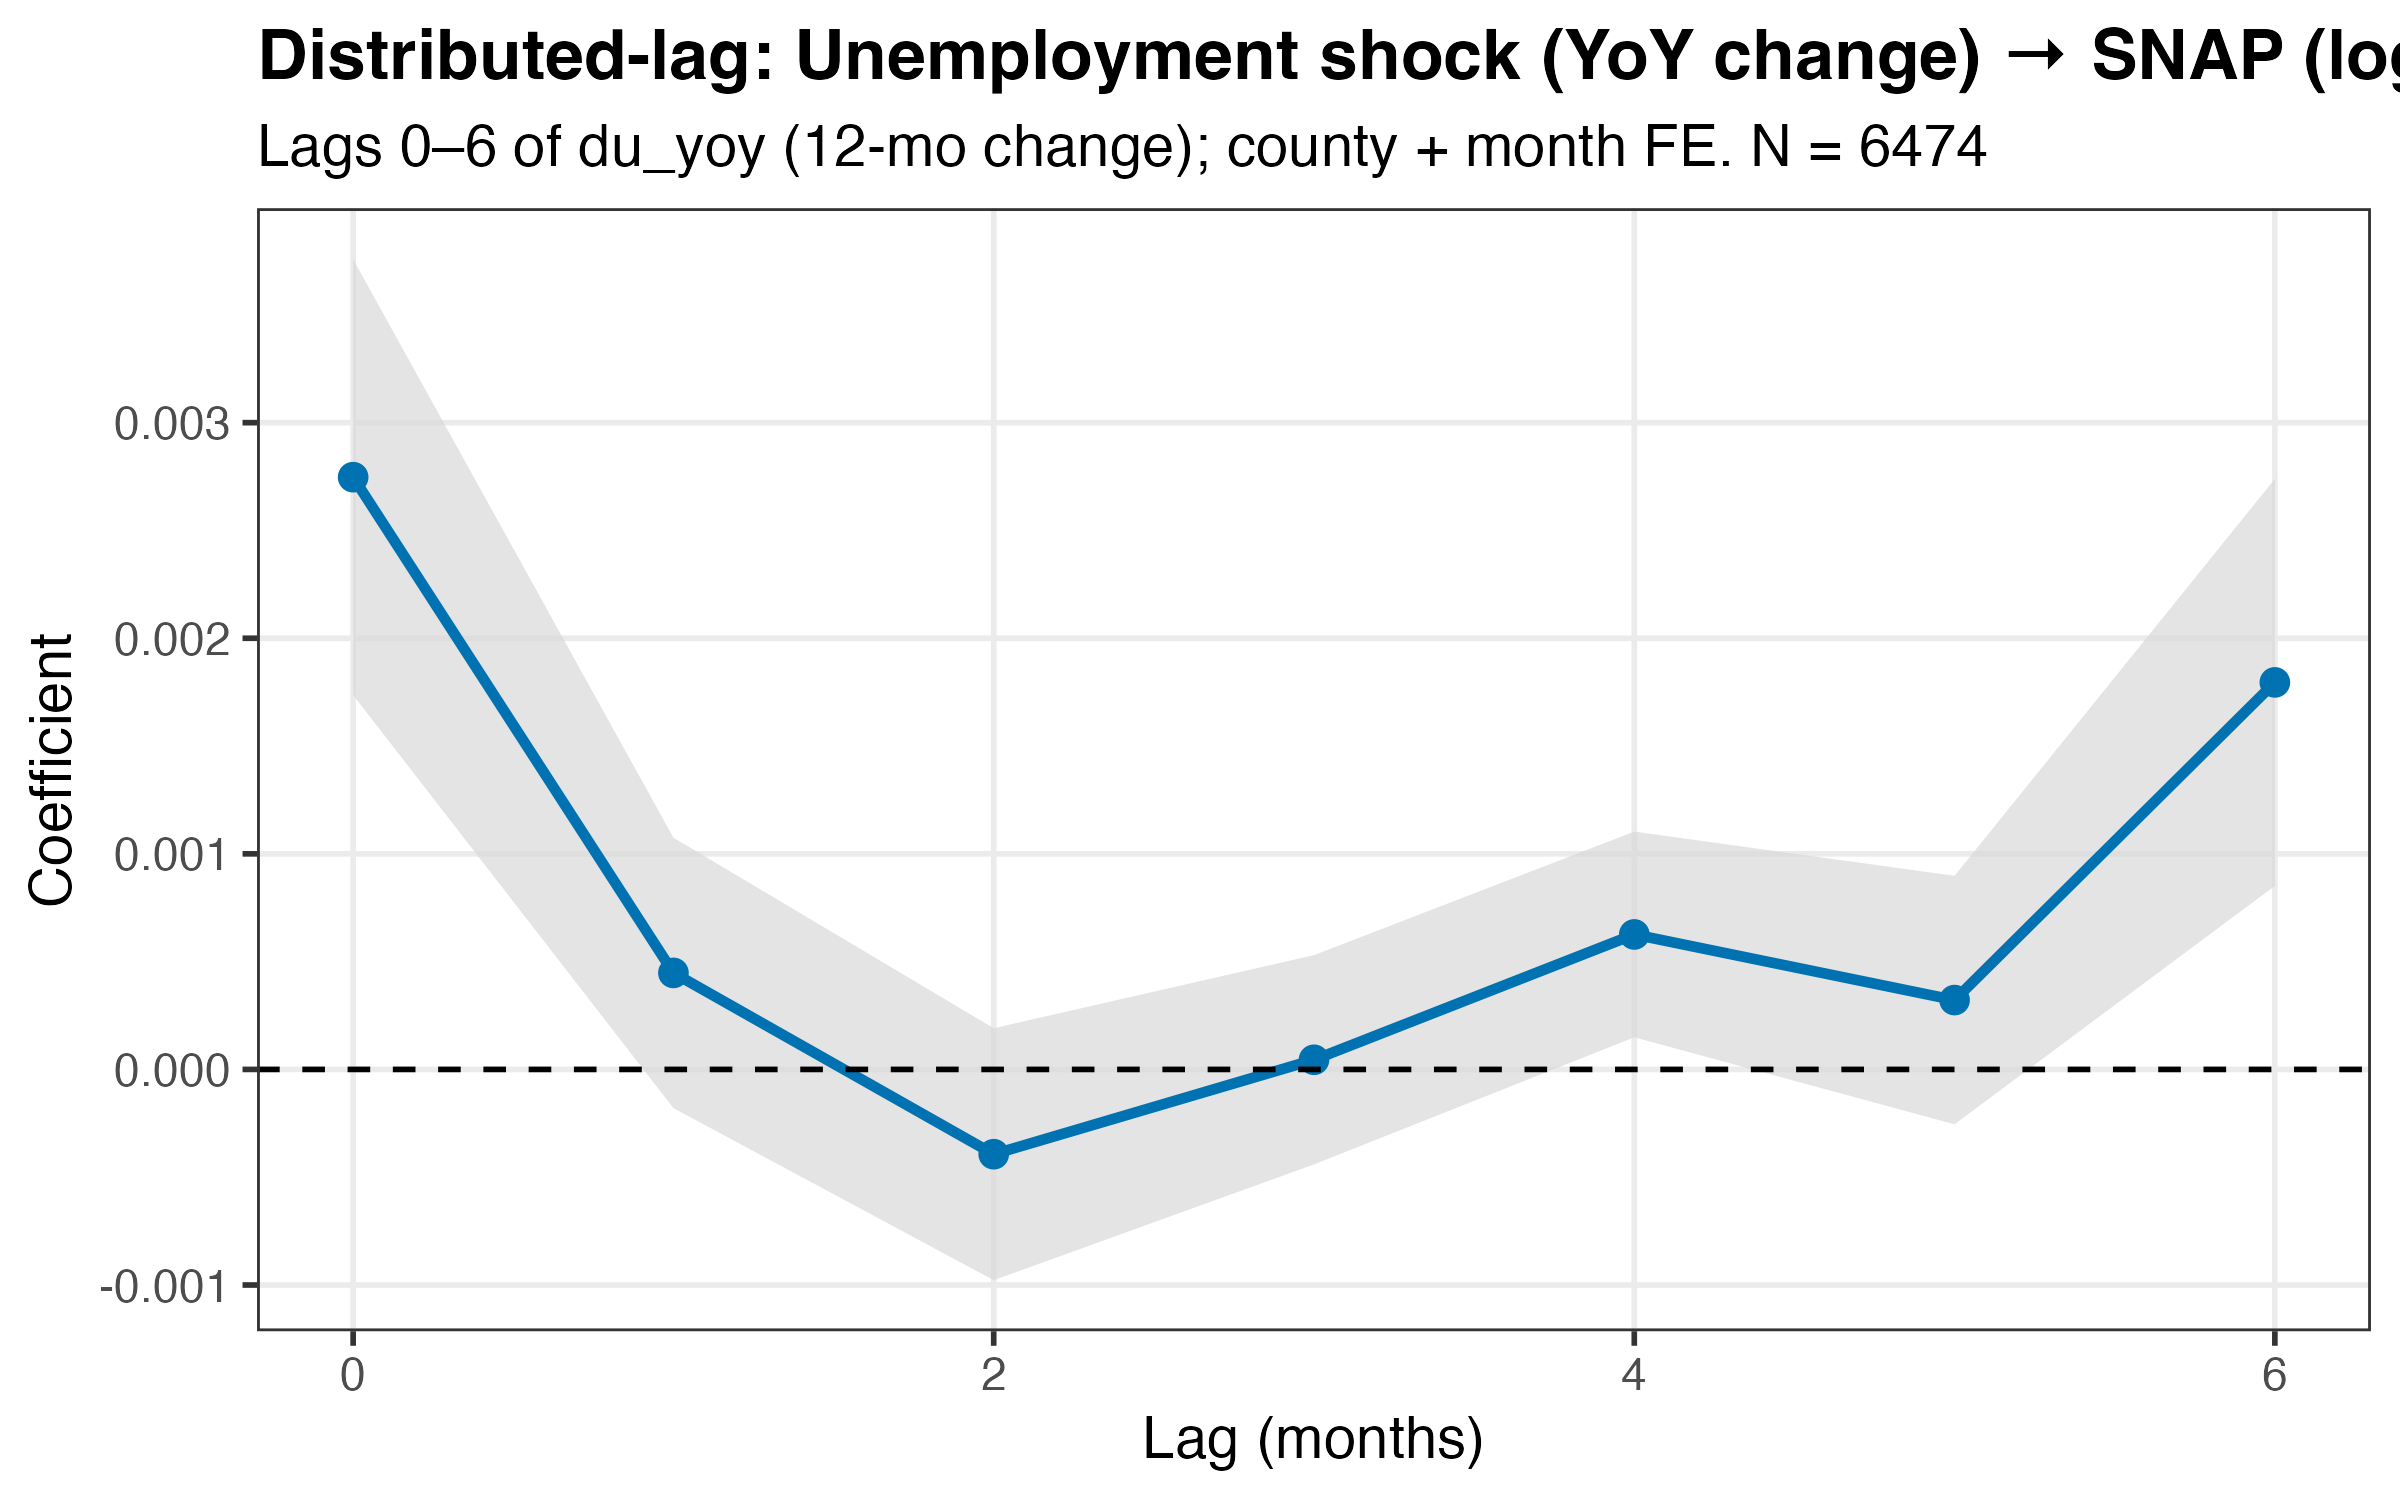
\includegraphics[width=0.85\textwidth]{../outputs/figures/income_dl_recipients}
%   \caption{Distributed-lag: dynamic response of SNAP participation (log 1+ recipients) to 12-month change in unemployment rate. County and month FE; lags 0--6; 95\% CI; SE clustered by county.}
%   \label{fig:income-dl}
% \end{figure}

% \begin{table}[htbp]
%   \centering
%   \caption{Distributed-lag estimates (income DL). Cumulative effect $\sum \beta$ reported in heterogeneity table.}
%   \label{tab:income-dl}
%   \input{../outputs/tables/income_dl_main}  % or manually type key rows
% \end{table}

% ---------------------------------------------------------------------------
\subsection{End of Emergency Allotments (EA) event study}
\label{sec:ea}

Event time is defined in integer months relative to the EA end (March 2023):
\begin{equation}
\text{event time}_t = (12 \times \text{year}_t + \text{month}_t) - (12 \times \text{year}_{\text{EA}} + \text{month}_{\text{EA}}).
\end{equation}

\paragraph{Average benefit (descriptive).}
We estimate $Y_{ct} = \alpha_c + \sum_{k \neq -1} \delta_k \,\mathbf{1}(\text{event time}_t = k) + \varepsilon_{ct}$ for average benefit per person, with $k=-1$ as reference. This documents the drop in benefits at the EA end.

% \begin{figure}[htbp]
%   \centering
%   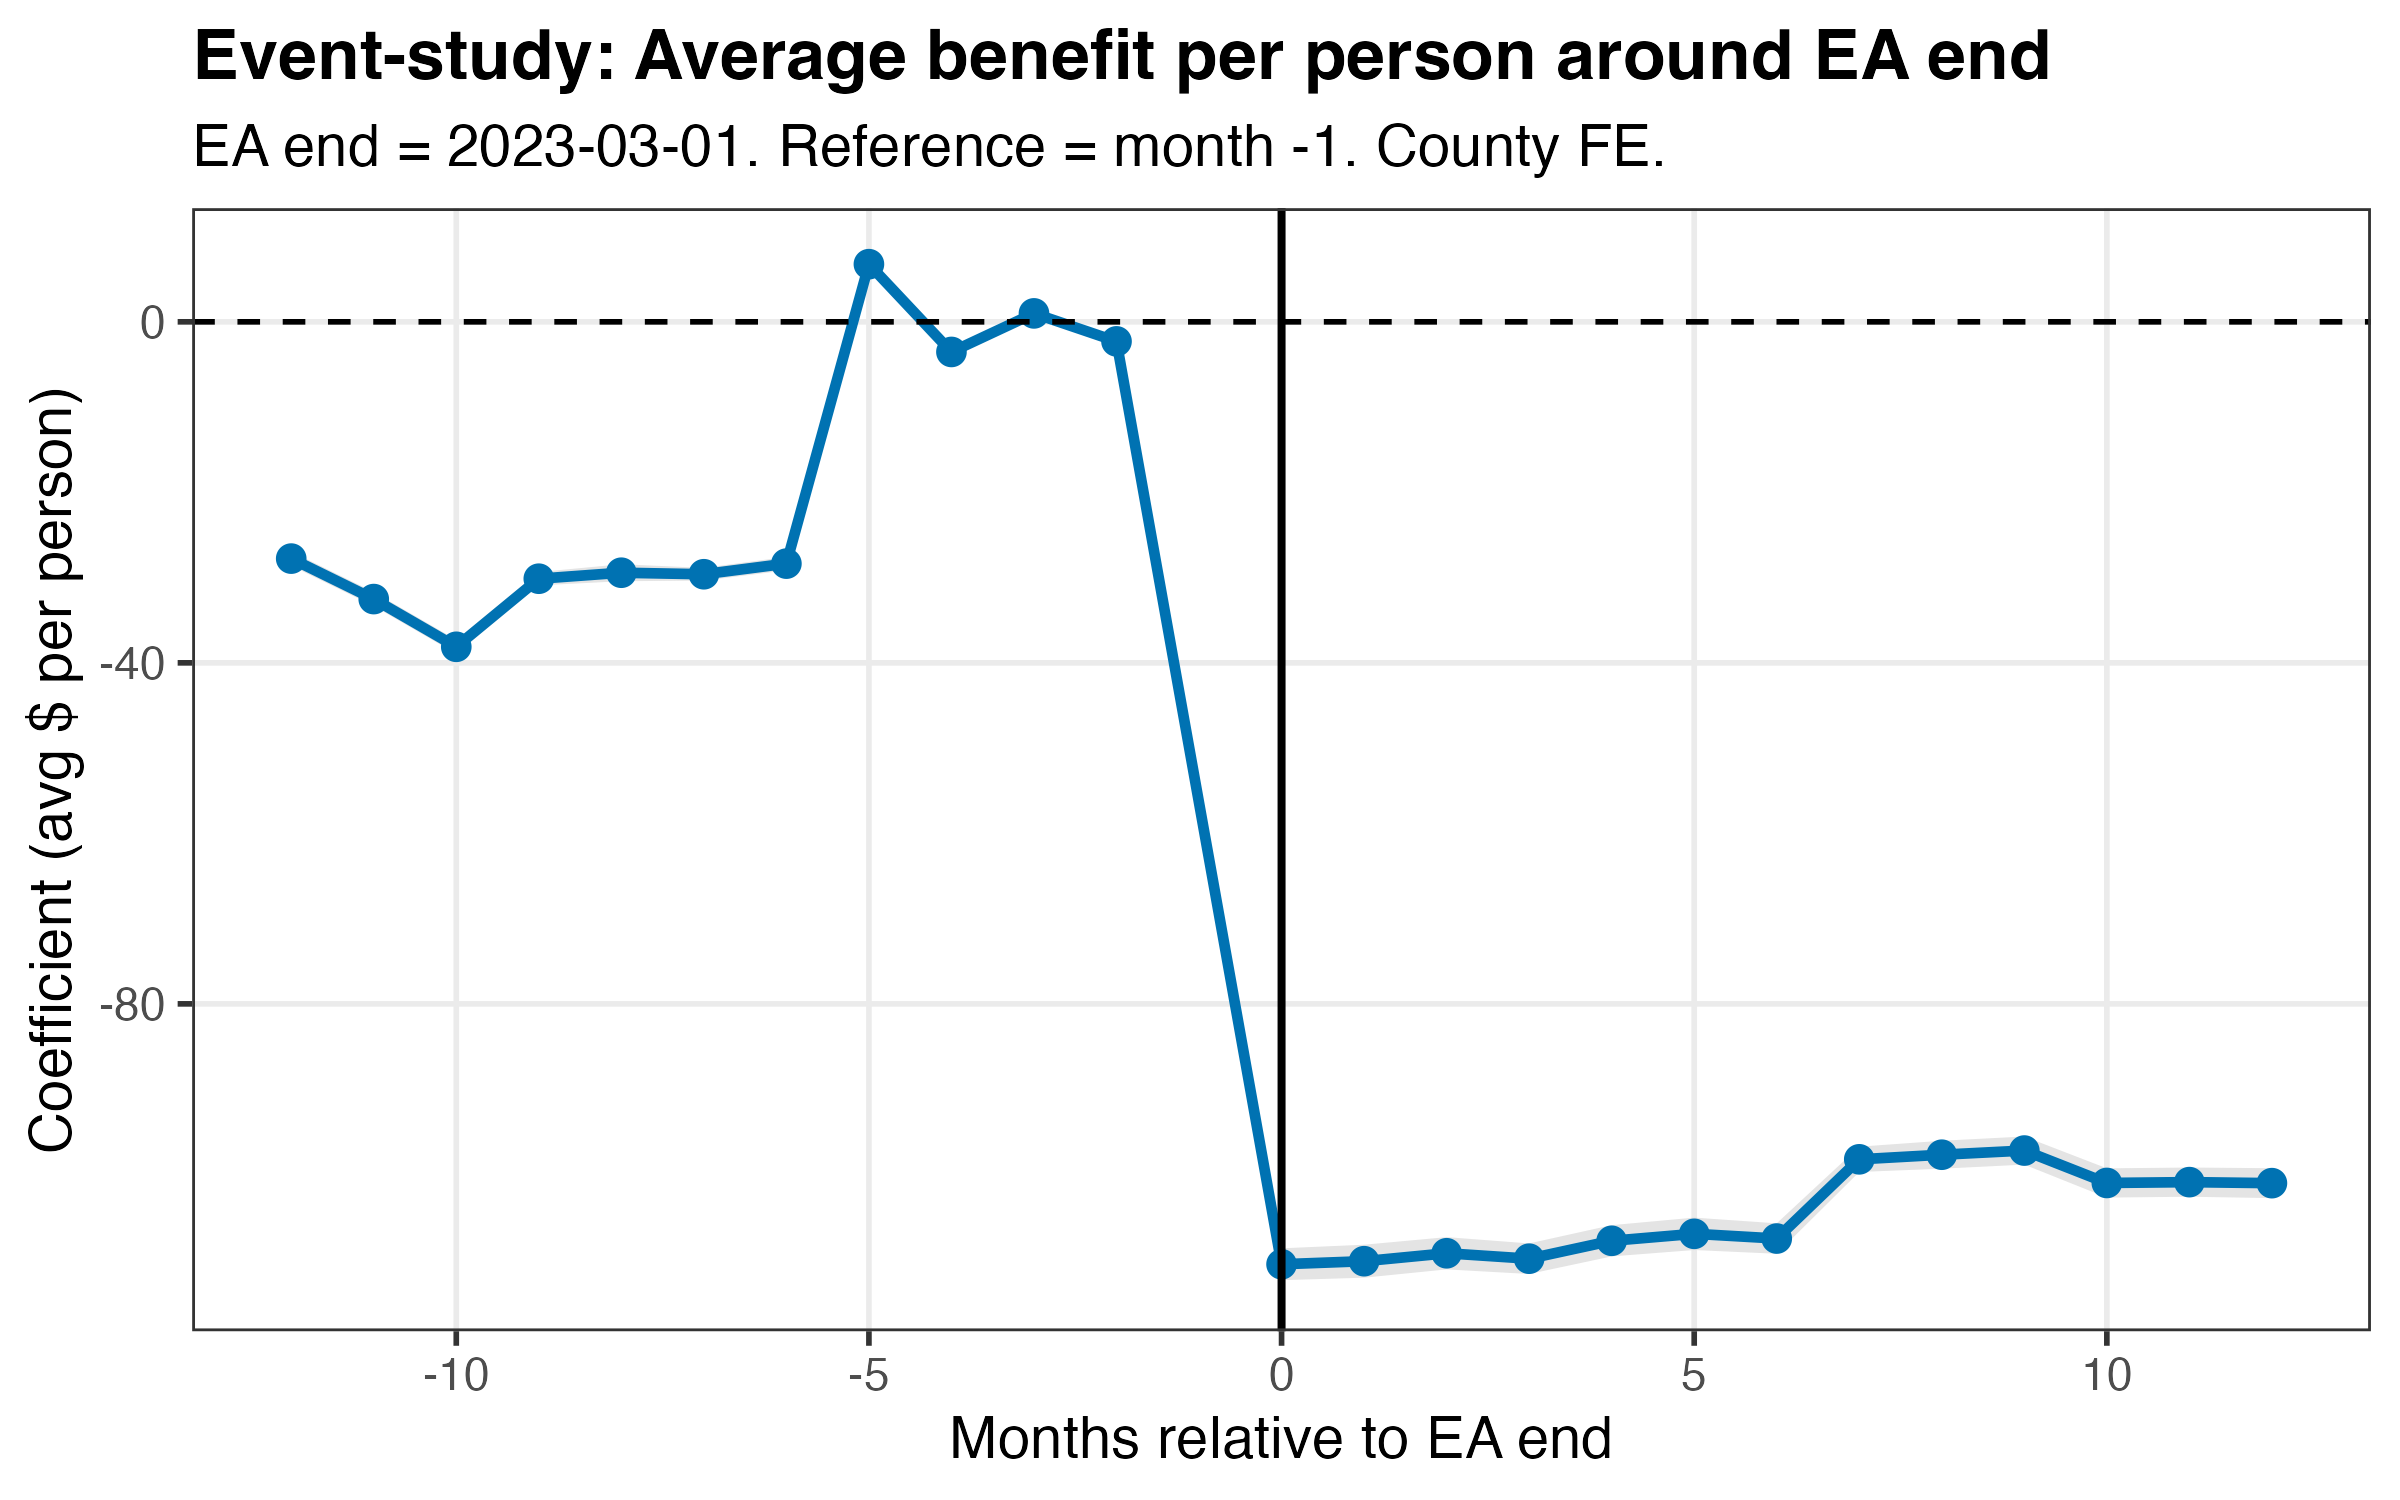
\includegraphics[width=0.85\textwidth]{../outputs/figures/ea_es_avgpp}
%   \caption{Event-study: average benefit per person around EA end. Reference month $-1$; county FE; 95\% CI.}
%   \label{fig:ea-avgpp}
% \end{figure}

\paragraph{Participation: intensity differential (main).}
For participation, we use a differential event-study with month fixed effects. Counties are classified as high or low ``intensity'' by whether their pre-EA (months $-12$ to $-1$) average benefit per person is above the median. We estimate
\begin{equation}
Y_{ct} = \alpha_c + \gamma_t + \sum_{k \neq -1} \theta_k \,\big(\mathbf{1}(\text{event time}_t = k) \times \text{High intensity}_c\big) + \varepsilon_{ct},
\end{equation}
where $\gamma_t$ are month fixed effects. Only the interaction terms are included; $\theta_k$ is the high-minus-low difference at event month $k$ (relative to $-1$), identifying the differential response under common time shocks.

% \begin{figure}[htbp]
%   \centering
%   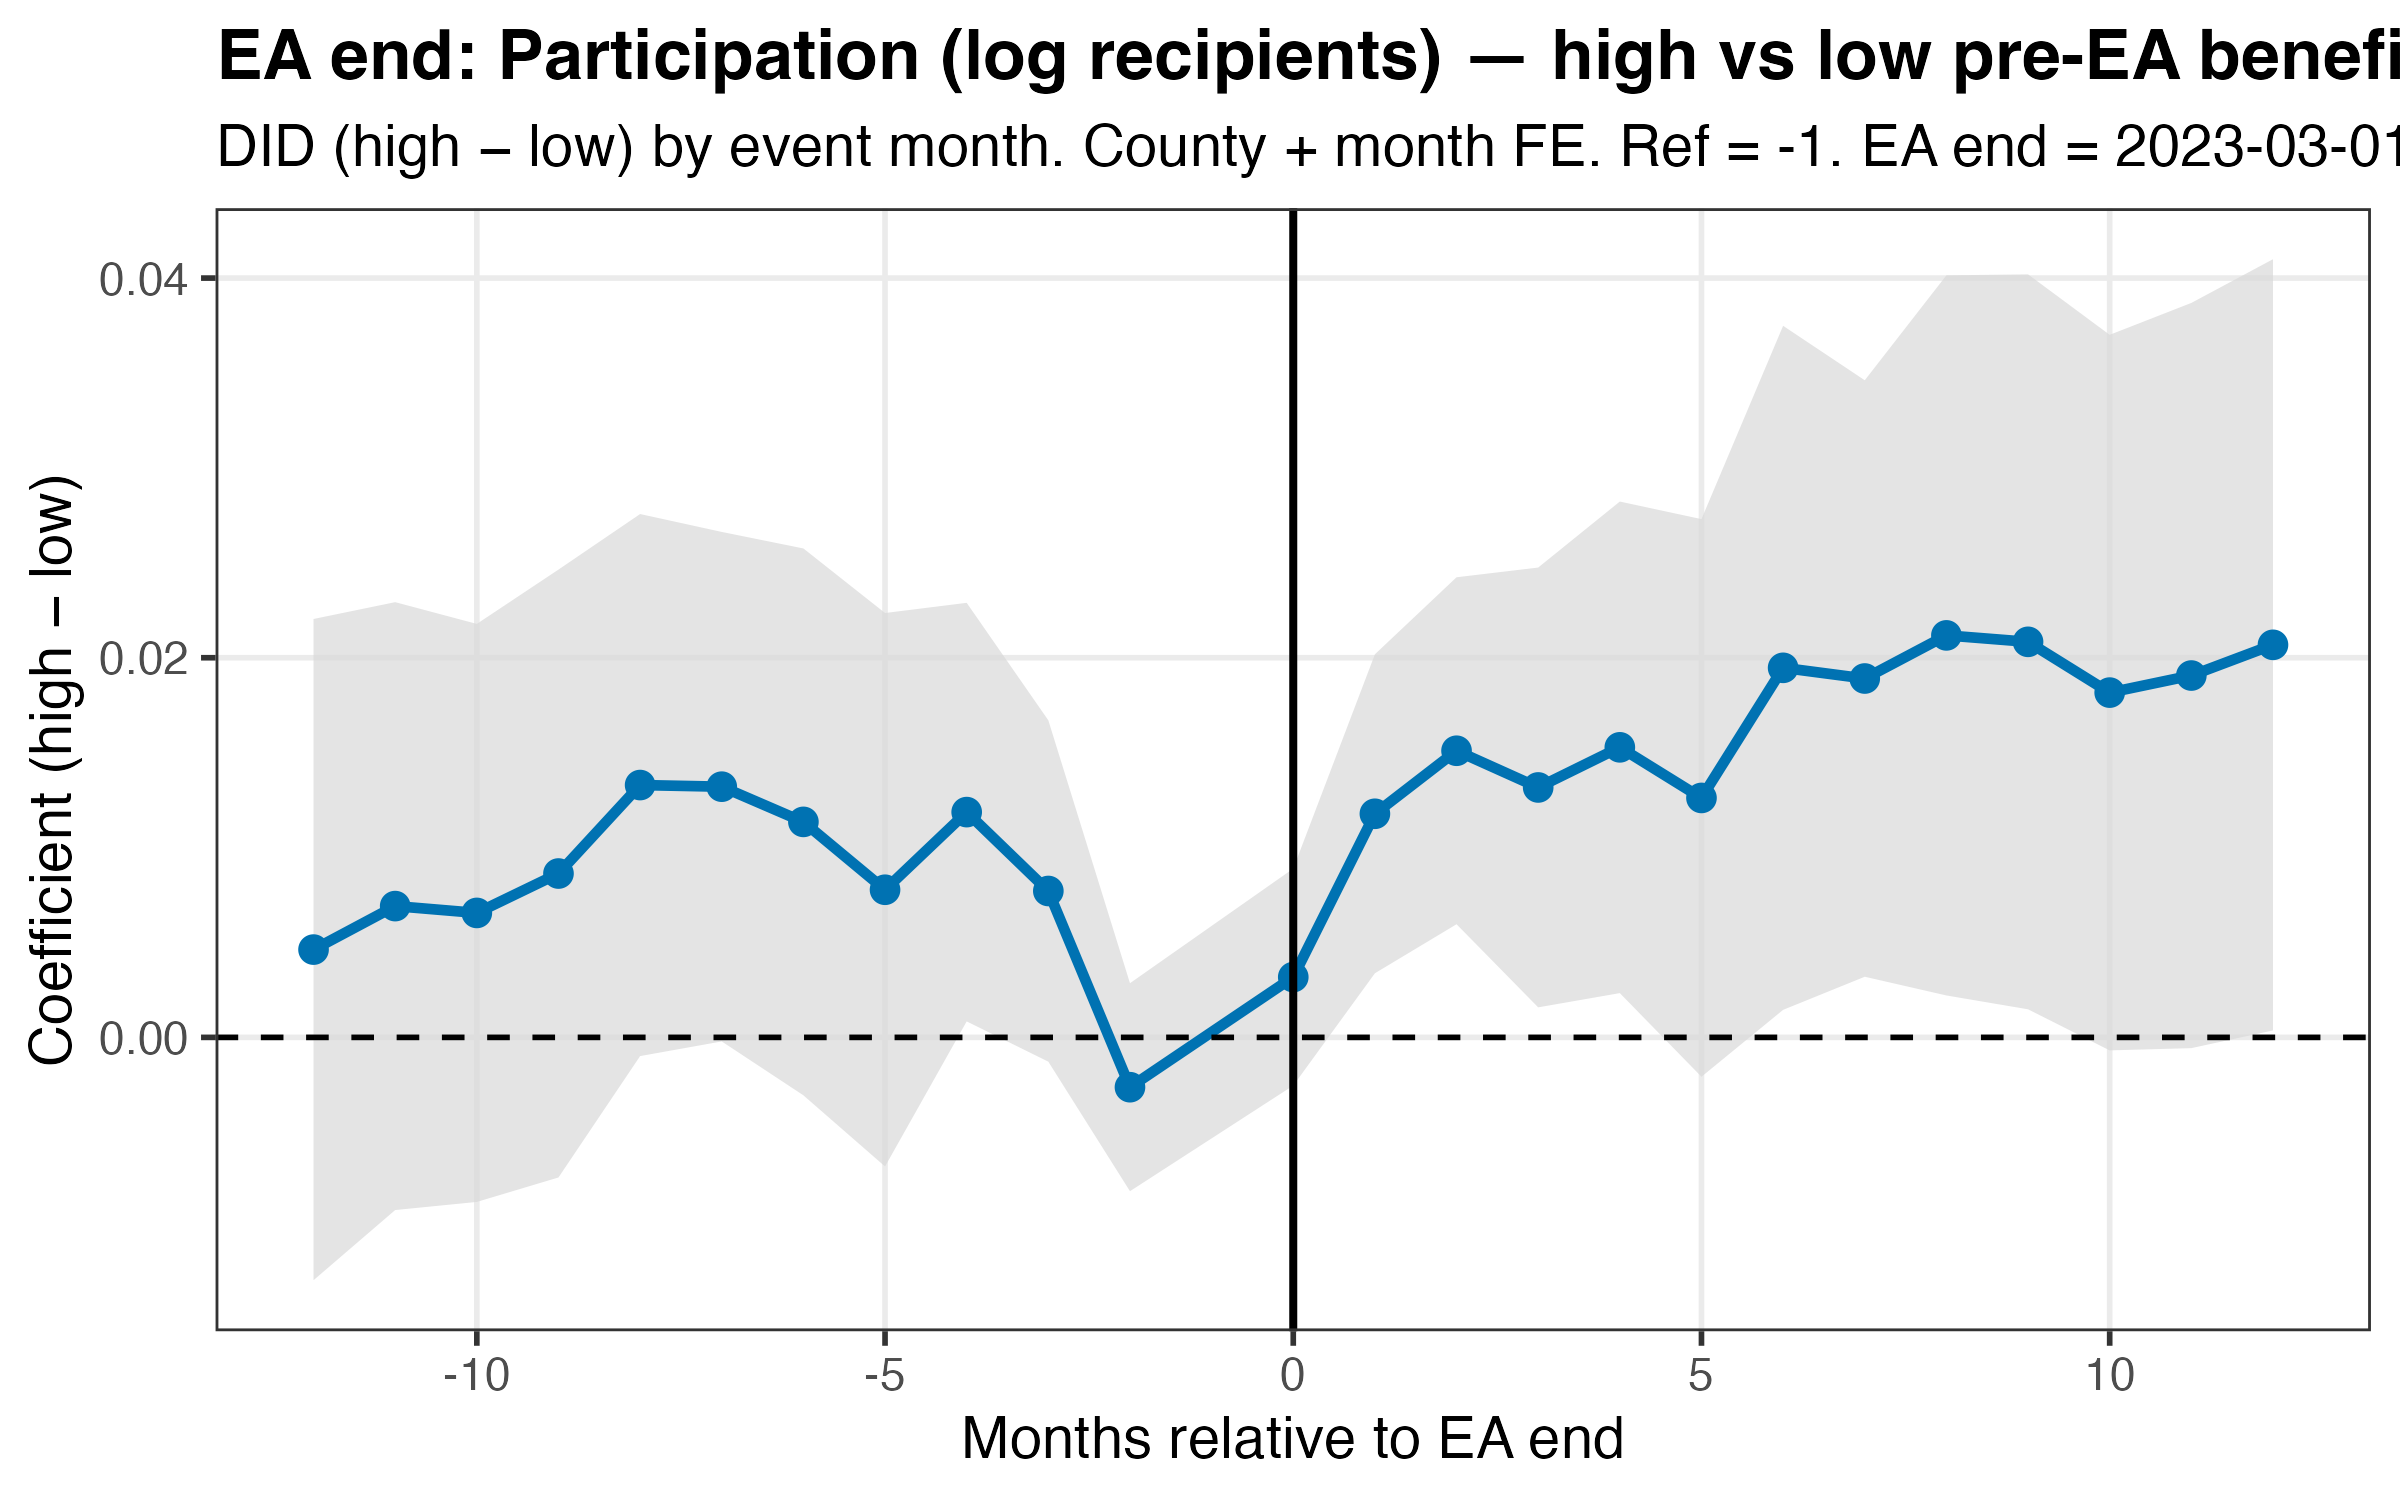
\includegraphics[width=0.85\textwidth]{../outputs/figures/ea_es_participation}
%   \caption{EA end: participation (log recipients), high vs.\ low pre-EA benefit intensity. Differential event-study (high $-$ low); county and month FE; ref.\ month $-1$; 95\% CI; SE clustered by county.}
%   \label{fig:ea-participation}
% \end{figure}

Appendix Table~\ref{tab:ea-heterogeneity-app} reports pre/post mean outcomes by intensity group (descriptive).

% Requires: \usepackage{amsmath,amssymb}

\subsection{Unemployment and SNAP participation (distributed lag)}
\label{sec:income-dl}

We estimate the dynamic response of SNAP participation to \emph{changes} in local unemployment using a distributed-lag (DL) specification in county--month panel data. The regressor is the 12-month change in the unemployment rate, $\Delta u_{ct} = u_{ct} - u_{c,t-12}$, so that coefficients are interpretable as the impulse response to an unemployment shock.

For county $c$ and month $t$,
\begin{equation}
Y_{ct} = \alpha_c + \gamma_t + \sum_{\ell=0}^{L} \beta_\ell \, \Delta u_{c,t-\ell} + \varepsilon_{ct},
\end{equation}
where $Y_{ct} = \ln(1 + \text{recipients}_{ct})$; $\alpha_c$ and $\gamma_t$ are county and month fixed effects; and $L=6$. Standard errors are clustered at the county level. The cumulative effect of a one percentage-point increase in the unemployment rate is $\sum_{\ell=0}^{L} \beta_\ell$.

Heterogeneity is based on \emph{pre-determined} exposure: we split counties by their average unemployment rate over 2014--2016 (before the main ABAWD rollout). The same DL model is estimated separately in the high- and low-exposure subsamples.

% --- Uncomment and adjust figure/table numbers when you add the actual floats ---
% \begin{figure}[htbp]
%   \centering
%   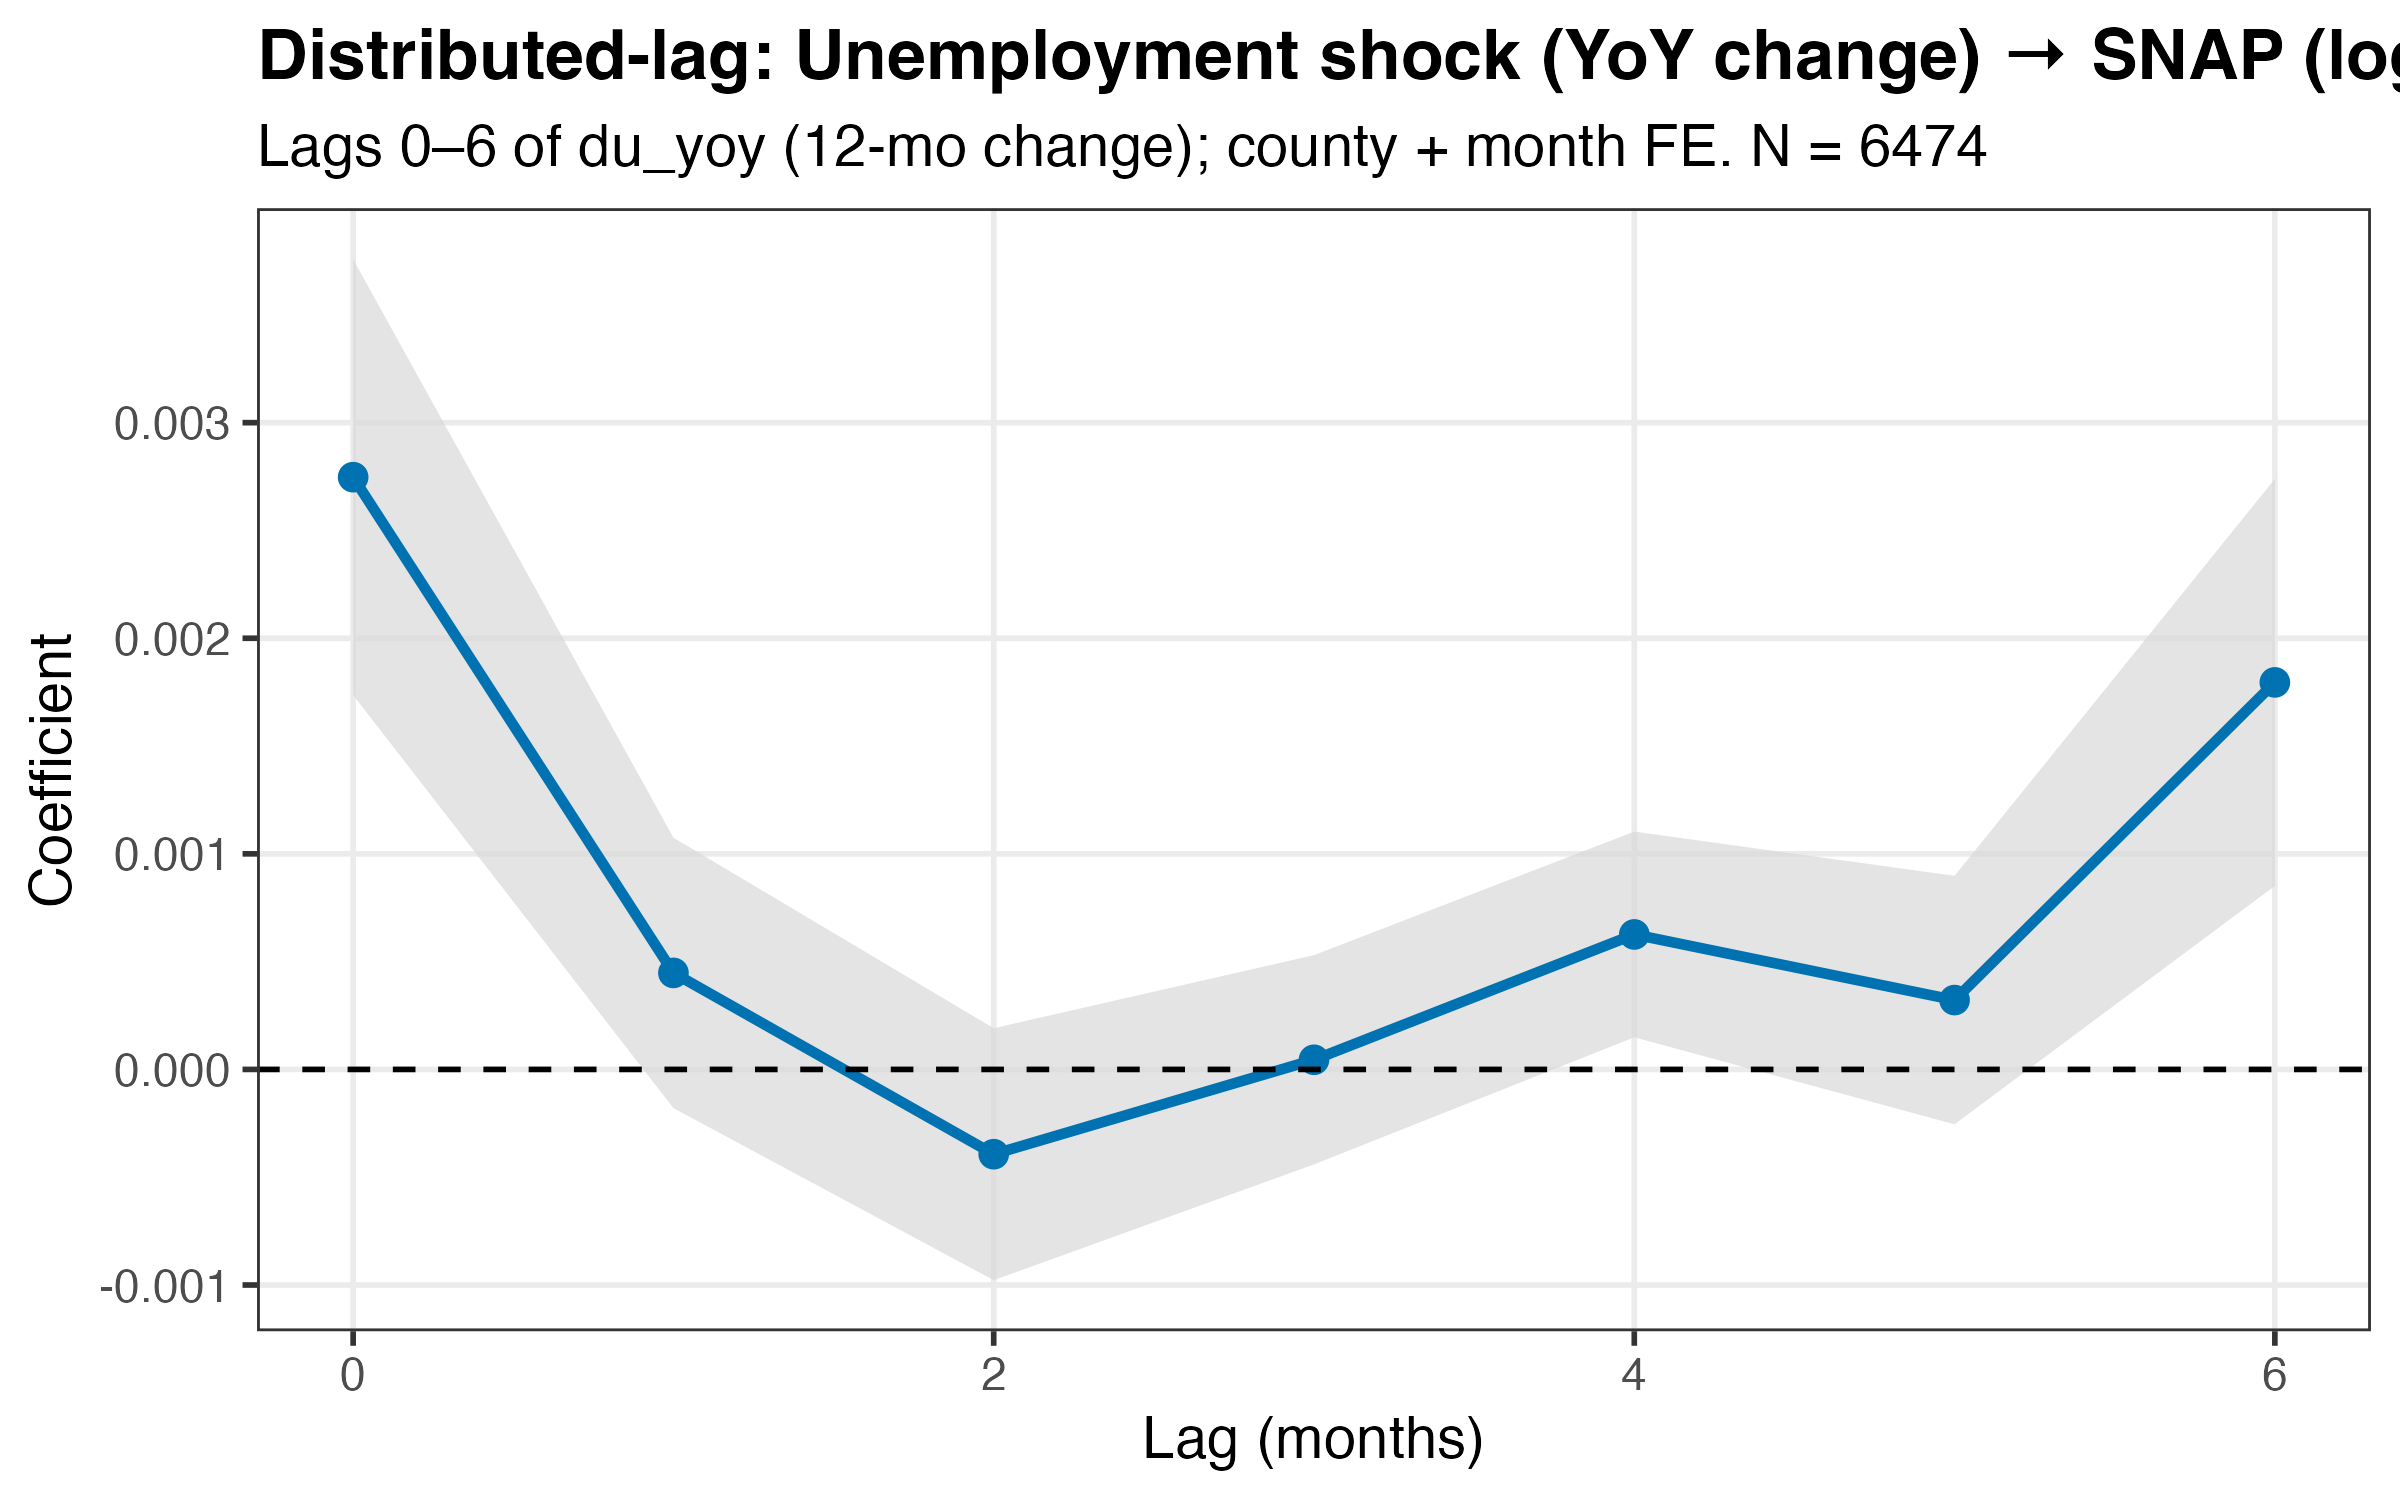
\includegraphics[width=0.85\textwidth]{../outputs/figures/income_dl_recipients}
%   \caption{Distributed-lag: dynamic response of SNAP participation (log 1+ recipients) to 12-month change in unemployment rate. County and month FE; lags 0--6; 95\% CI; SE clustered by county.}
%   \label{fig:income-dl}
% \end{figure}

% \begin{table}[htbp]
%   \centering
%   \caption{Distributed-lag estimates (income DL). Cumulative effect $\sum \beta$ reported in heterogeneity table.}
%   \label{tab:income-dl}
%   \input{../outputs/tables/income_dl_main}  % or manually type key rows
% \end{table}

% ---------------------------------------------------------------------------
\subsection{End of Emergency Allotments (EA) event study}
\label{sec:ea}

Event time is defined in integer months relative to the EA end (March 2023):
\begin{equation}
\text{event time}_t = (12 \times \text{year}_t + \text{month}_t) - (12 \times \text{year}_{\text{EA}} + \text{month}_{\text{EA}}).
\end{equation}

\paragraph{Average benefit (descriptive).}
We estimate $Y_{ct} = \alpha_c + \sum_{k \neq -1} \delta_k \,\mathbf{1}(\text{event time}_t = k) + \varepsilon_{ct}$ for average benefit per person, with $k=-1$ as reference. This documents the drop in benefits at the EA end.

% \begin{figure}[htbp]
%   \centering
%   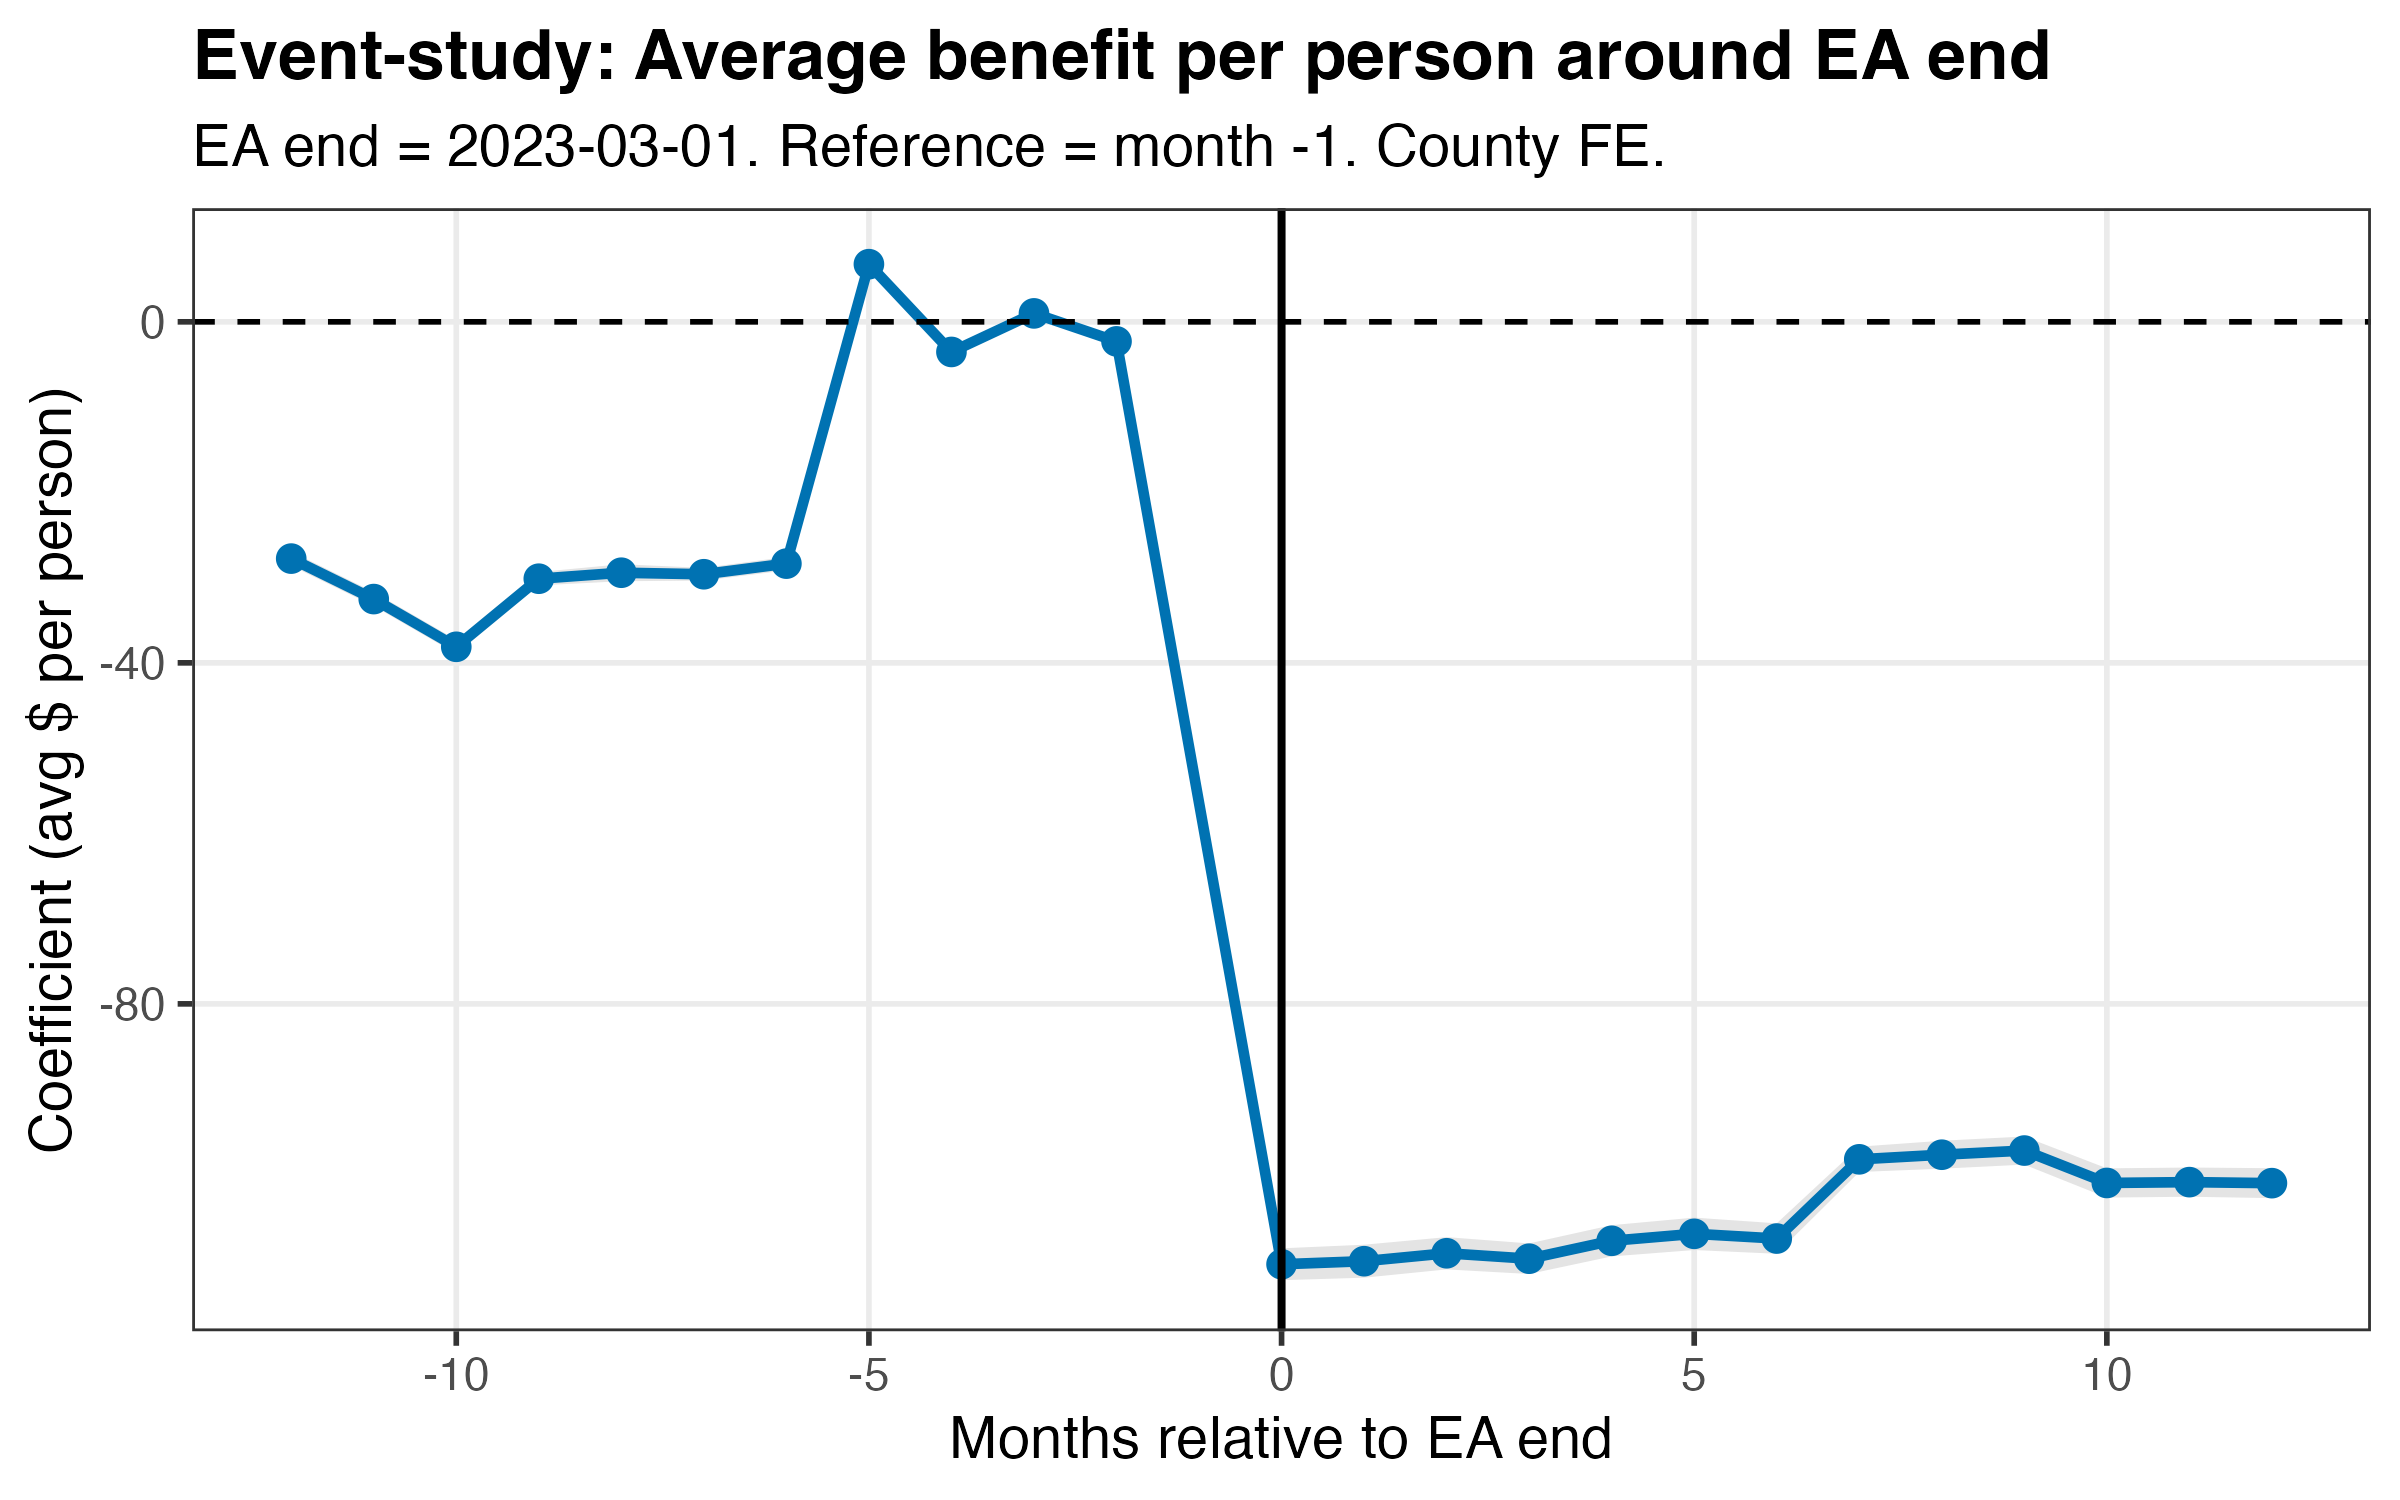
\includegraphics[width=0.85\textwidth]{../outputs/figures/ea_es_avgpp}
%   \caption{Event-study: average benefit per person around EA end. Reference month $-1$; county FE; 95\% CI.}
%   \label{fig:ea-avgpp}
% \end{figure}

\paragraph{Participation: intensity differential (main).}
For participation, we use a differential event-study with month fixed effects. Counties are classified as high or low ``intensity'' by whether their pre-EA (months $-12$ to $-1$) average benefit per person is above the median. We estimate
\begin{equation}
Y_{ct} = \alpha_c + \gamma_t + \sum_{k \neq -1} \theta_k \,\big(\mathbf{1}(\text{event time}_t = k) \times \text{High intensity}_c\big) + \varepsilon_{ct},
\end{equation}
where $\gamma_t$ are month fixed effects. Only the interaction terms are included; $\theta_k$ is the high-minus-low difference at event month $k$ (relative to $-1$), identifying the differential response under common time shocks.

% \begin{figure}[htbp]
%   \centering
%   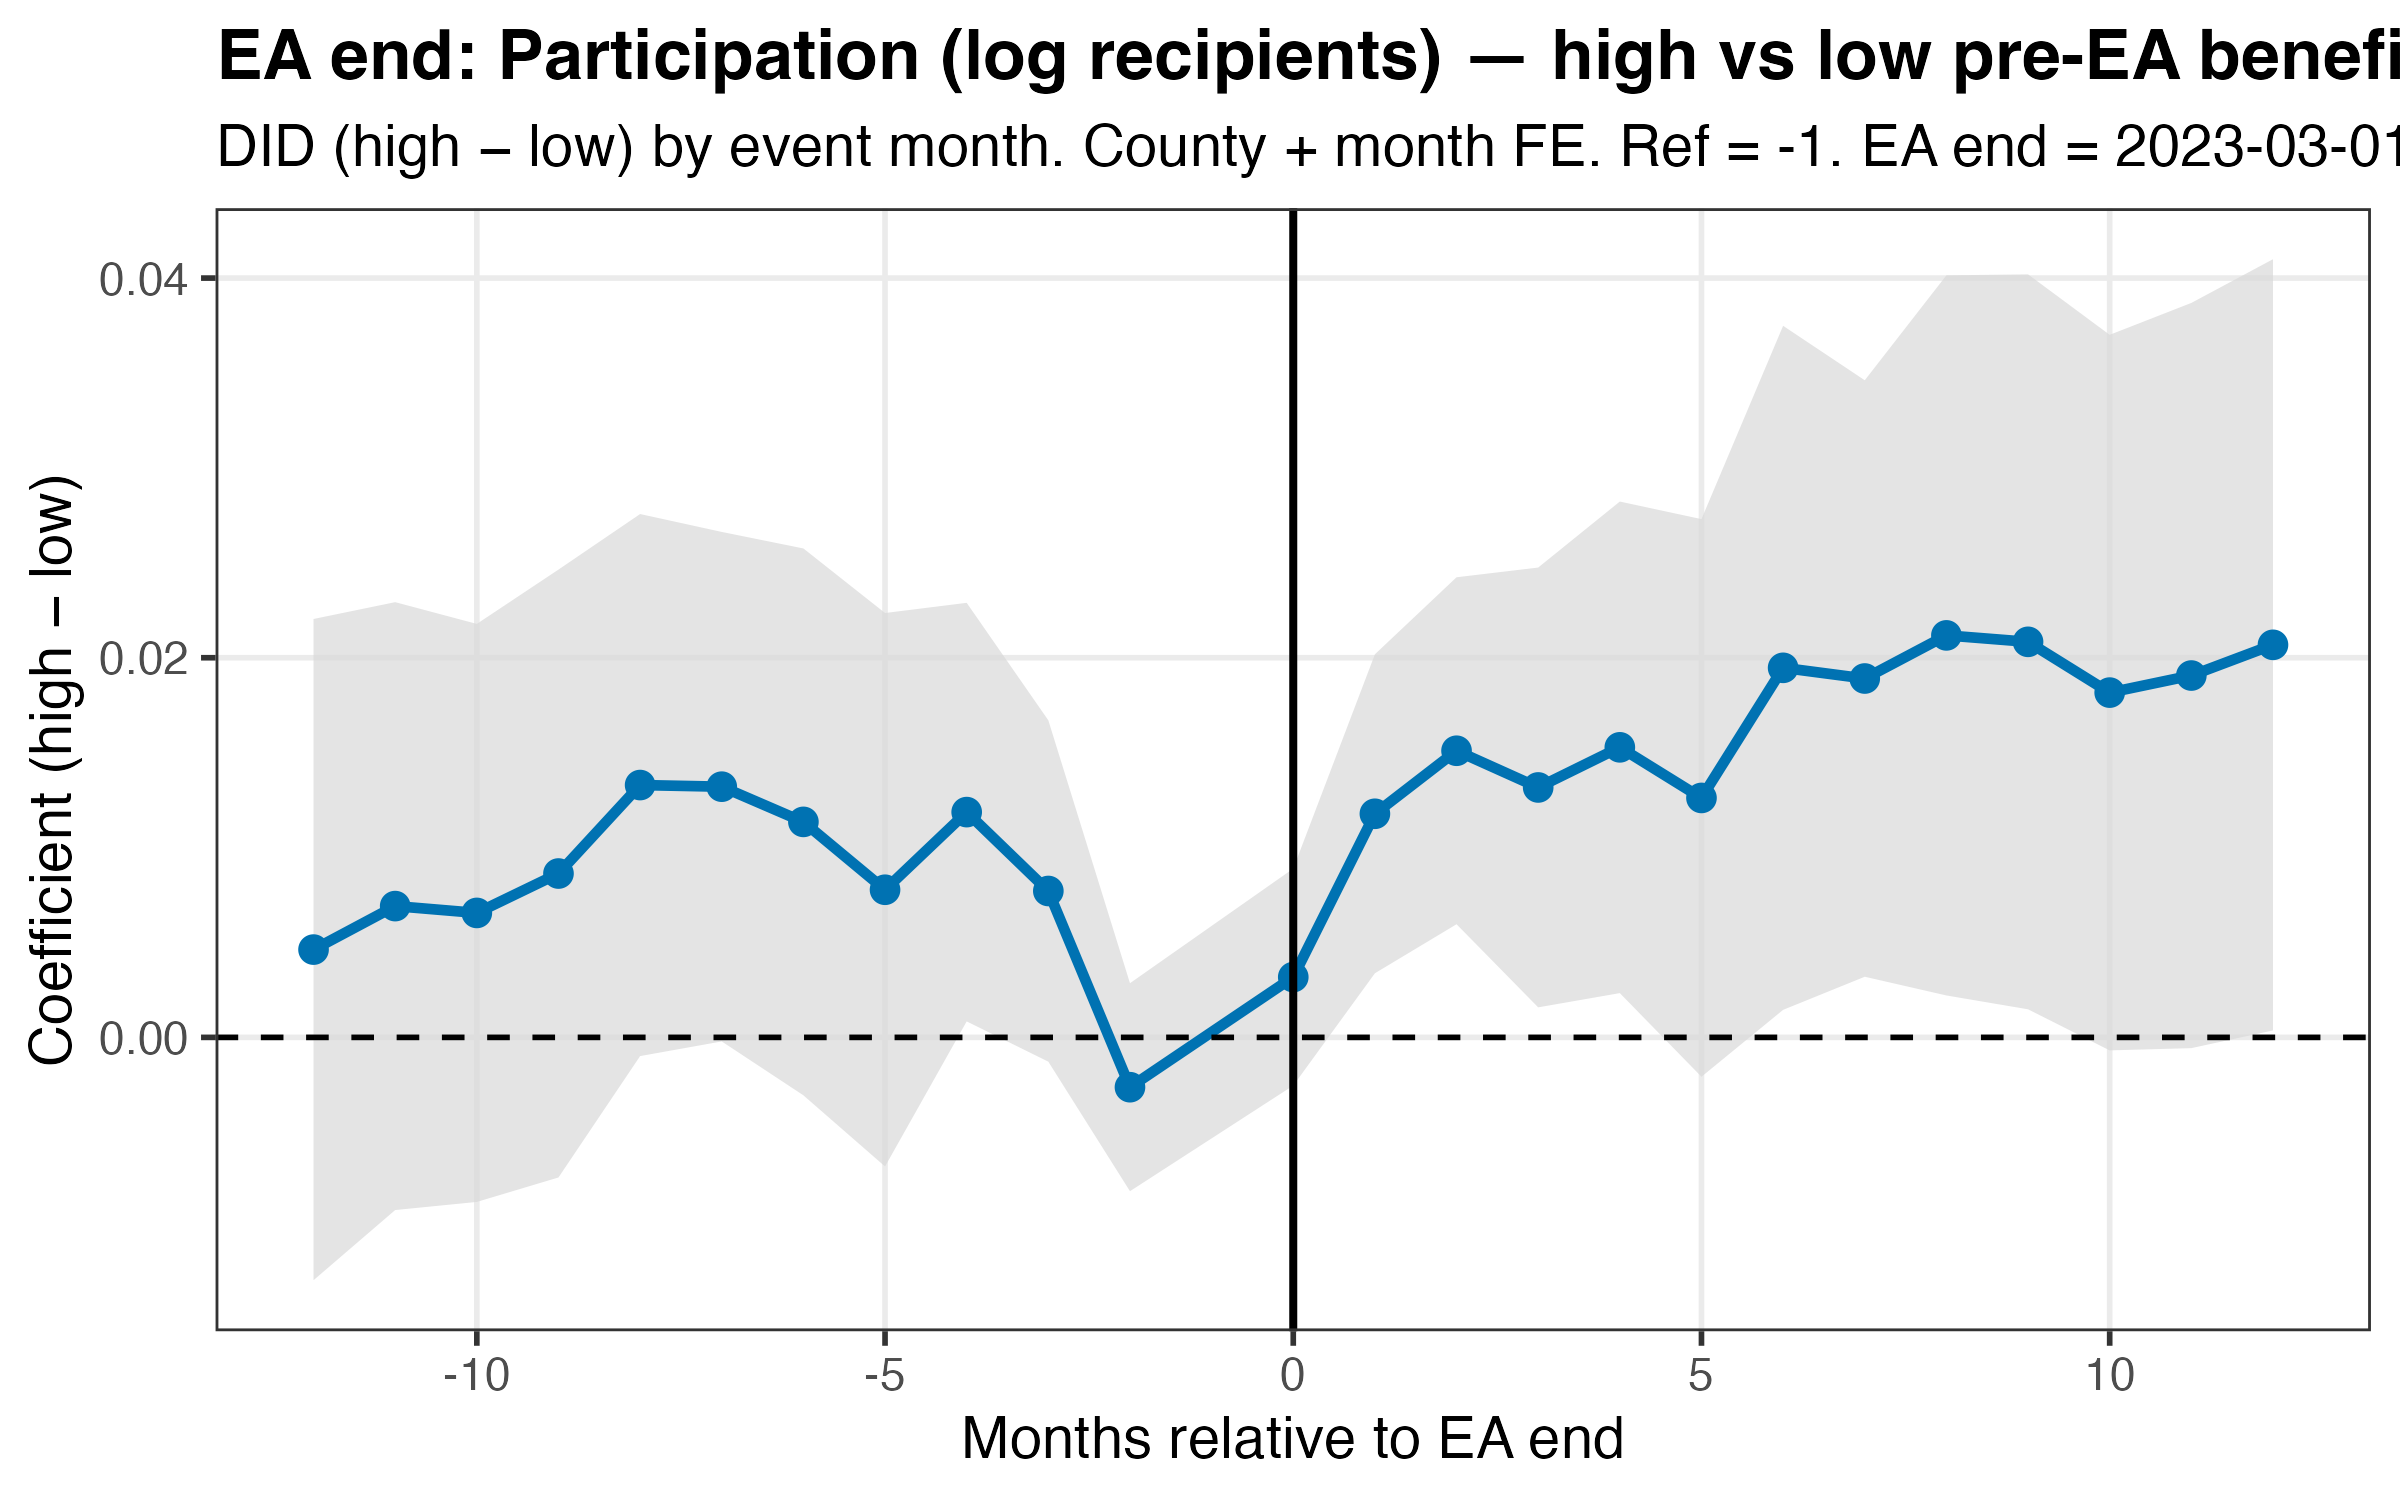
\includegraphics[width=0.85\textwidth]{../outputs/figures/ea_es_participation}
%   \caption{EA end: participation (log recipients), high vs.\ low pre-EA benefit intensity. Differential event-study (high $-$ low); county and month FE; ref.\ month $-1$; 95\% CI; SE clustered by county.}
%   \label{fig:ea-participation}
% \end{figure}

Appendix Table~\ref{tab:ea-heterogeneity-app} reports pre/post mean outcomes by intensity group (descriptive).

% Requires: \usepackage{amsmath,amssymb}

\subsection{Unemployment and SNAP participation (distributed lag)}
\label{sec:income-dl}

We estimate the dynamic response of SNAP participation to \emph{changes} in local unemployment using a distributed-lag (DL) specification in county--month panel data. The regressor is the 12-month change in the unemployment rate, $\Delta u_{ct} = u_{ct} - u_{c,t-12}$, so that coefficients are interpretable as the impulse response to an unemployment shock.

For county $c$ and month $t$,
\begin{equation}
Y_{ct} = \alpha_c + \gamma_t + \sum_{\ell=0}^{L} \beta_\ell \, \Delta u_{c,t-\ell} + \varepsilon_{ct},
\end{equation}
where $Y_{ct} = \ln(1 + \text{recipients}_{ct})$; $\alpha_c$ and $\gamma_t$ are county and month fixed effects; and $L=6$. Standard errors are clustered at the county level. The cumulative effect of a one percentage-point increase in the unemployment rate is $\sum_{\ell=0}^{L} \beta_\ell$.

Heterogeneity is based on \emph{pre-determined} exposure: we split counties by their average unemployment rate over 2014--2016 (before the main ABAWD rollout). The same DL model is estimated separately in the high- and low-exposure subsamples.

% --- Uncomment and adjust figure/table numbers when you add the actual floats ---
% \begin{figure}[htbp]
%   \centering
%   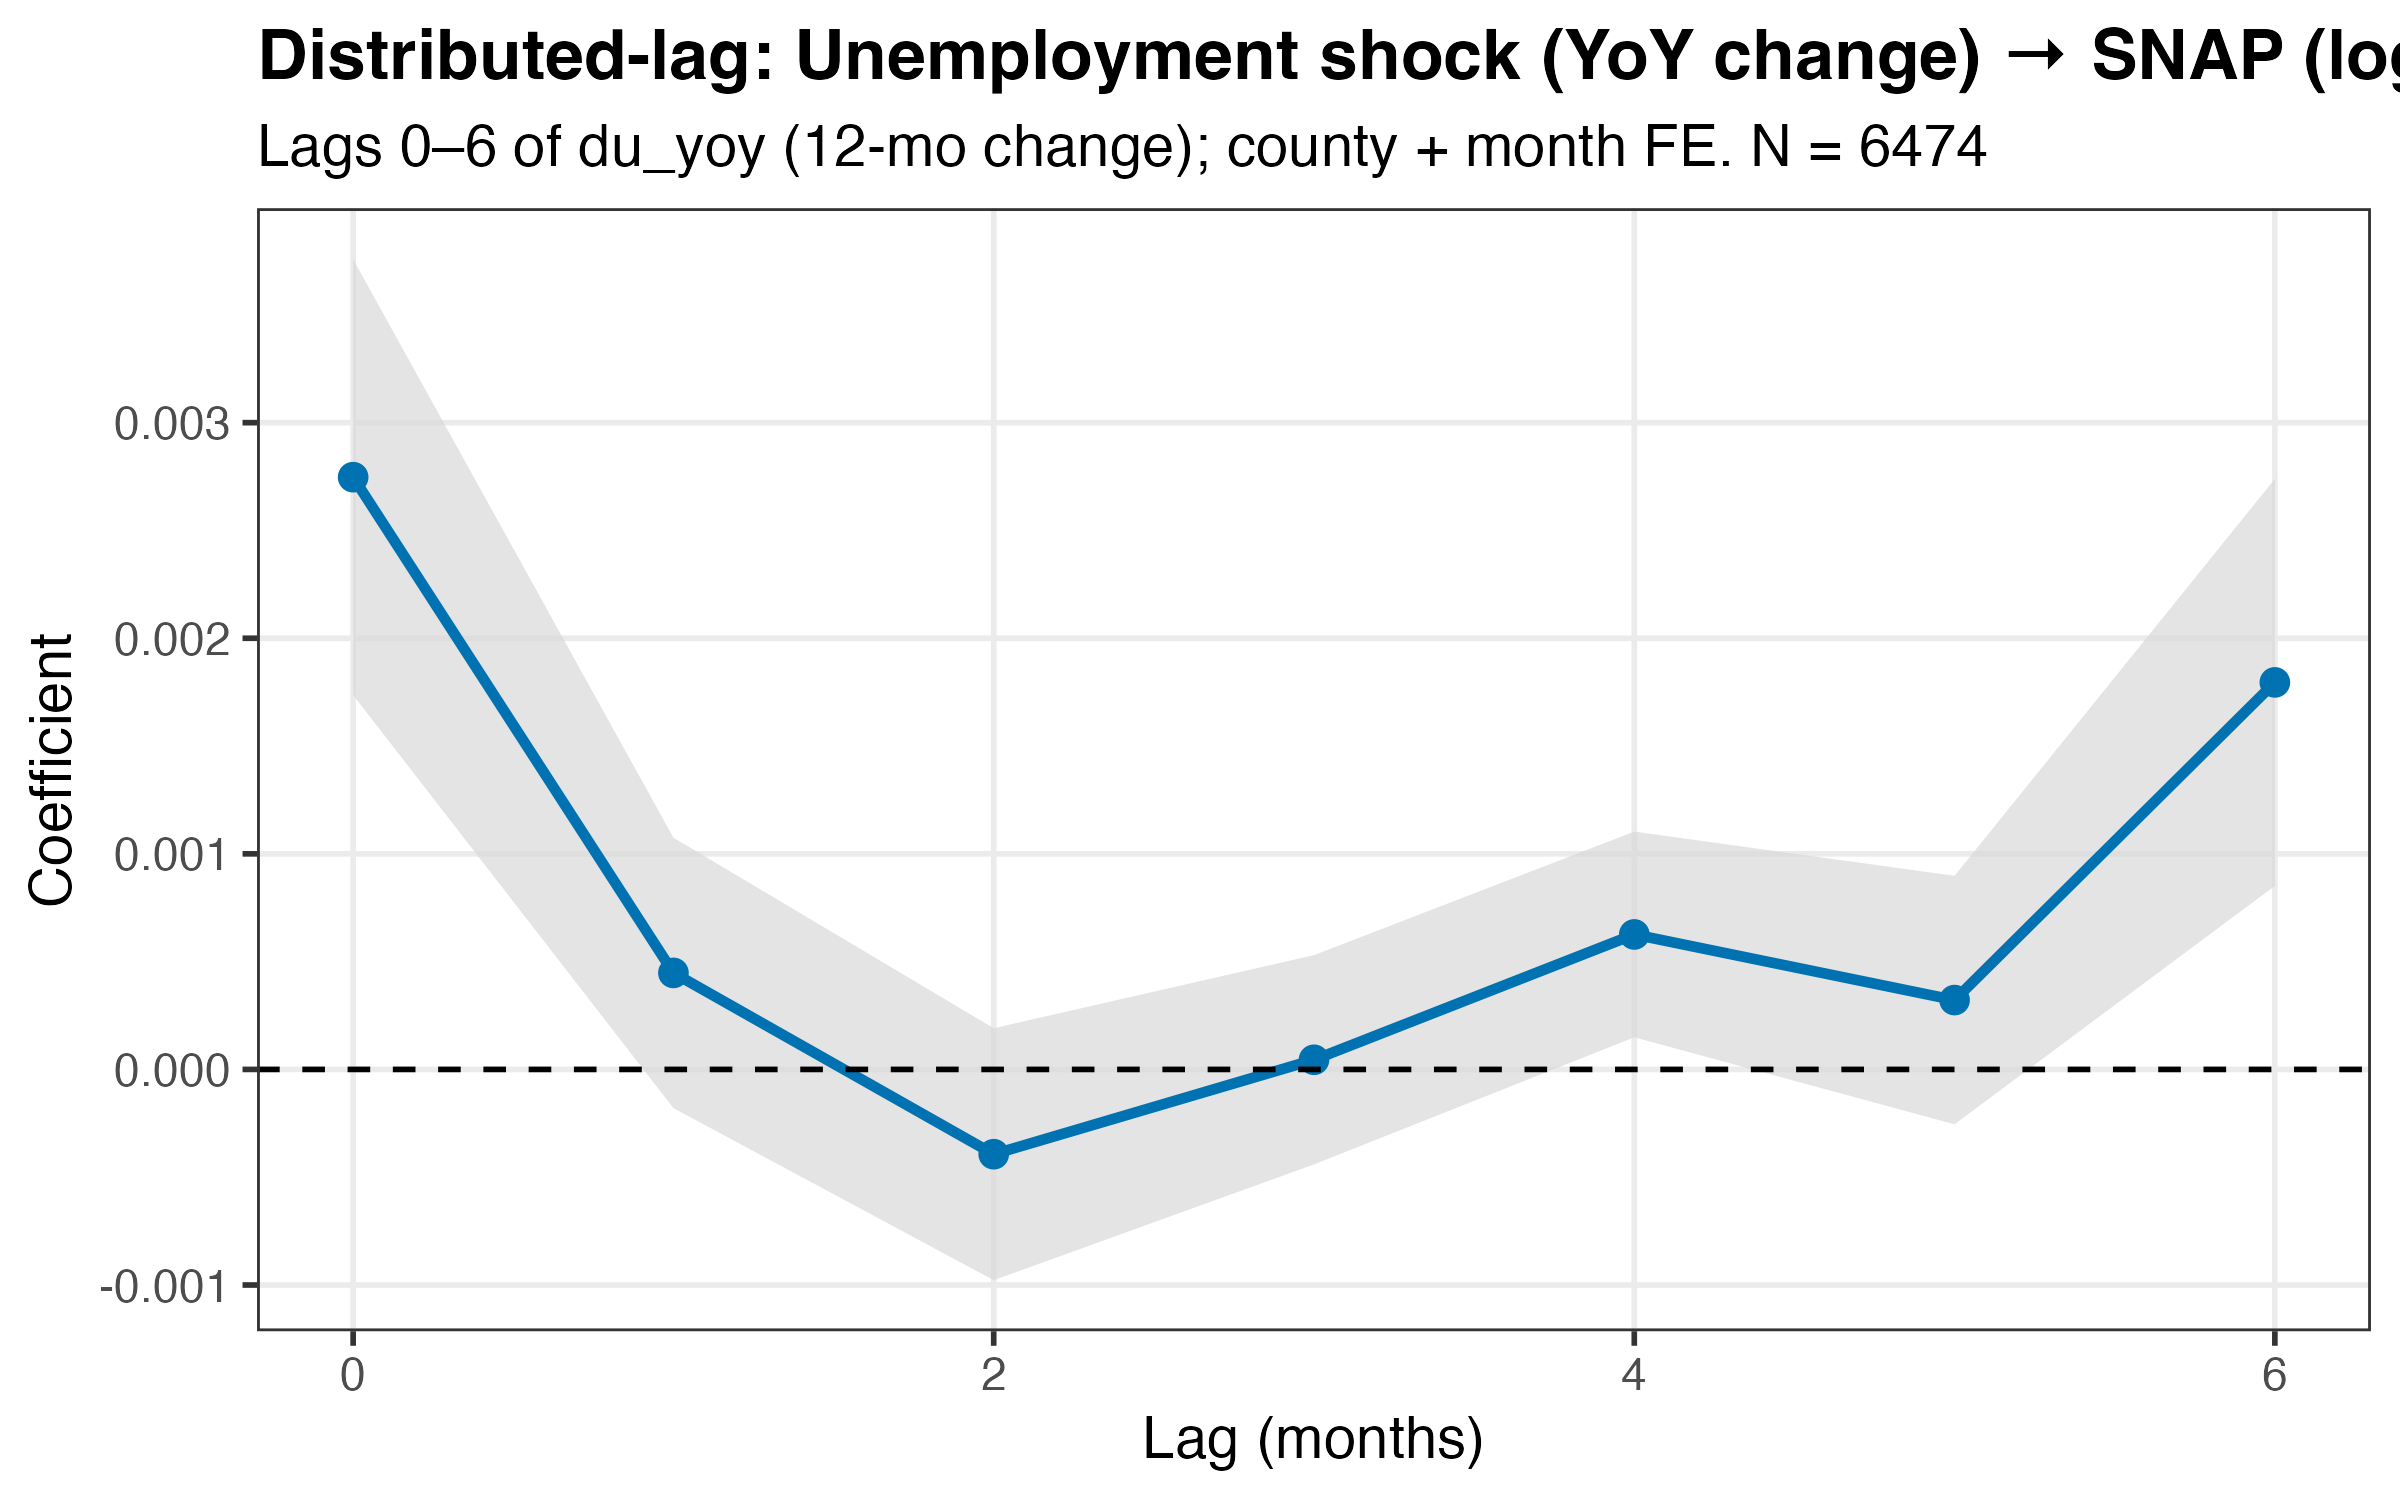
\includegraphics[width=0.85\textwidth]{../outputs/figures/income_dl_recipients}
%   \caption{Distributed-lag: dynamic response of SNAP participation (log 1+ recipients) to 12-month change in unemployment rate. County and month FE; lags 0--6; 95\% CI; SE clustered by county.}
%   \label{fig:income-dl}
% \end{figure}

% \begin{table}[htbp]
%   \centering
%   \caption{Distributed-lag estimates (income DL). Cumulative effect $\sum \beta$ reported in heterogeneity table.}
%   \label{tab:income-dl}
%   \input{../outputs/tables/income_dl_main}  % or manually type key rows
% \end{table}

% ---------------------------------------------------------------------------
\subsection{End of Emergency Allotments (EA) event study}
\label{sec:ea}

Event time is defined in integer months relative to the EA end (March 2023):
\begin{equation}
\text{event time}_t = (12 \times \text{year}_t + \text{month}_t) - (12 \times \text{year}_{\text{EA}} + \text{month}_{\text{EA}}).
\end{equation}

\paragraph{Average benefit (descriptive).}
We estimate $Y_{ct} = \alpha_c + \sum_{k \neq -1} \delta_k \,\mathbf{1}(\text{event time}_t = k) + \varepsilon_{ct}$ for average benefit per person, with $k=-1$ as reference. This documents the drop in benefits at the EA end.

% \begin{figure}[htbp]
%   \centering
%   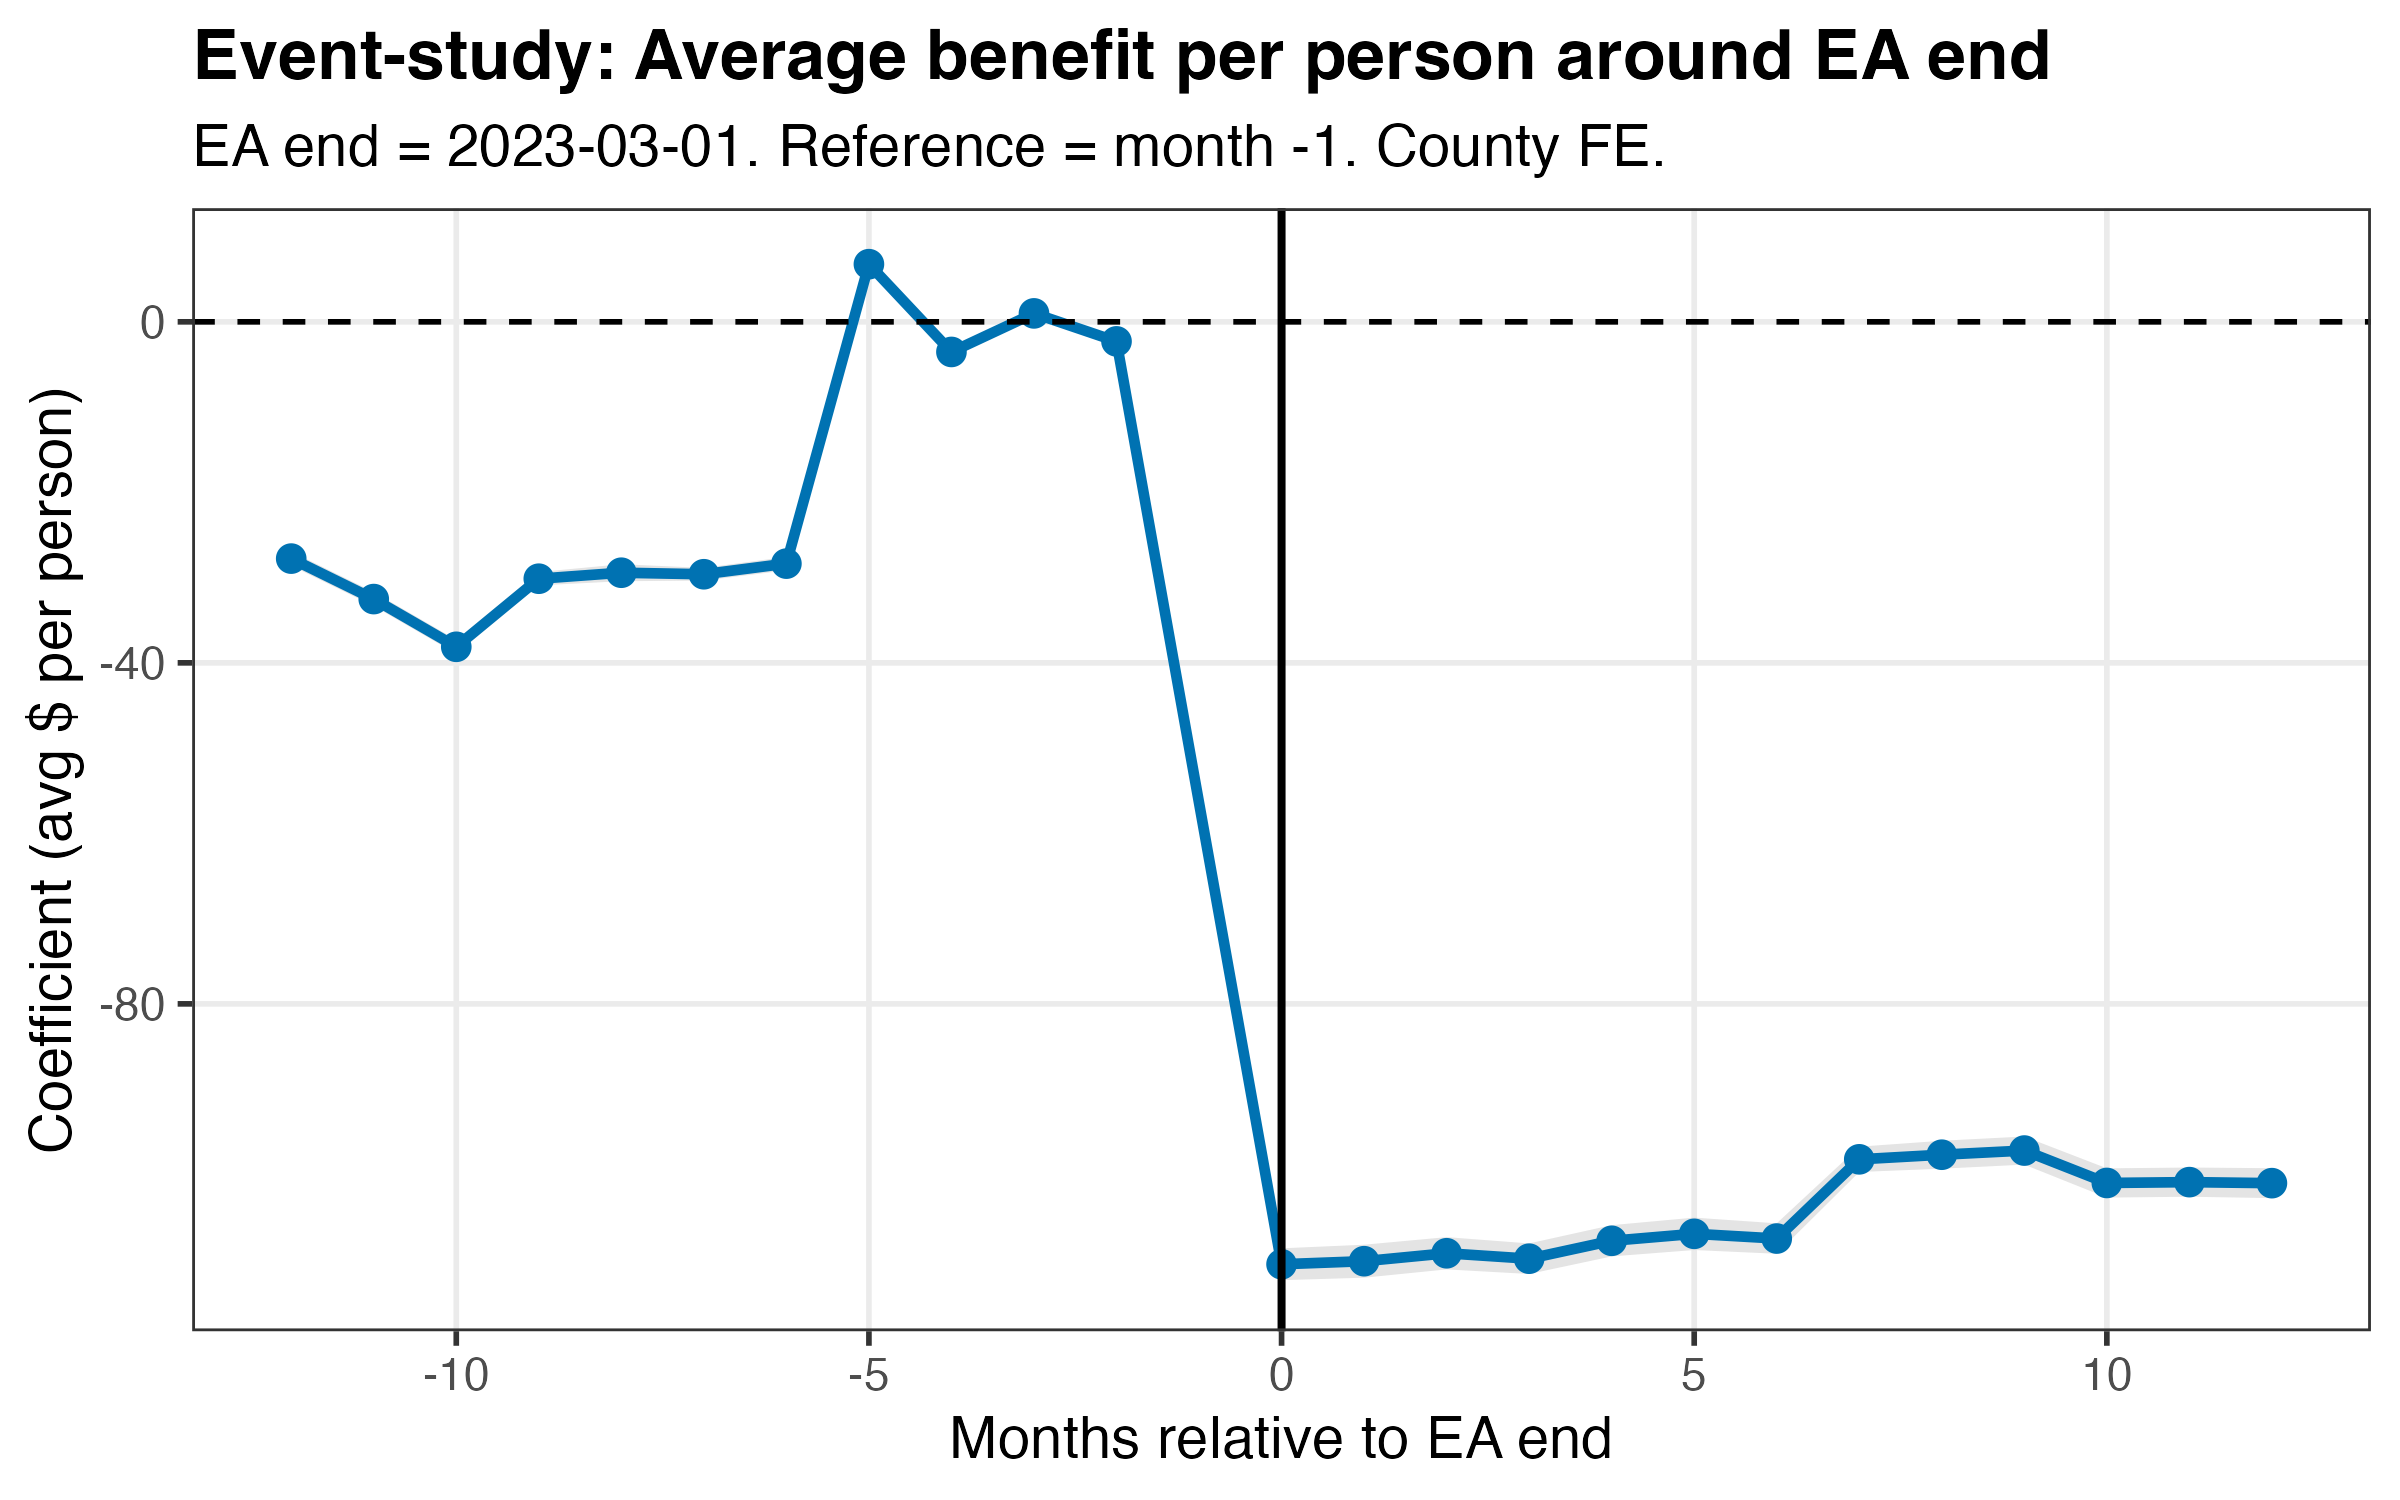
\includegraphics[width=0.85\textwidth]{../outputs/figures/ea_es_avgpp}
%   \caption{Event-study: average benefit per person around EA end. Reference month $-1$; county FE; 95\% CI.}
%   \label{fig:ea-avgpp}
% \end{figure}

\paragraph{Participation: intensity differential (main).}
For participation, we use a differential event-study with month fixed effects. Counties are classified as high or low ``intensity'' by whether their pre-EA (months $-12$ to $-1$) average benefit per person is above the median. We estimate
\begin{equation}
Y_{ct} = \alpha_c + \gamma_t + \sum_{k \neq -1} \theta_k \,\big(\mathbf{1}(\text{event time}_t = k) \times \text{High intensity}_c\big) + \varepsilon_{ct},
\end{equation}
where $\gamma_t$ are month fixed effects. Only the interaction terms are included; $\theta_k$ is the high-minus-low difference at event month $k$ (relative to $-1$), identifying the differential response under common time shocks.

% \begin{figure}[htbp]
%   \centering
%   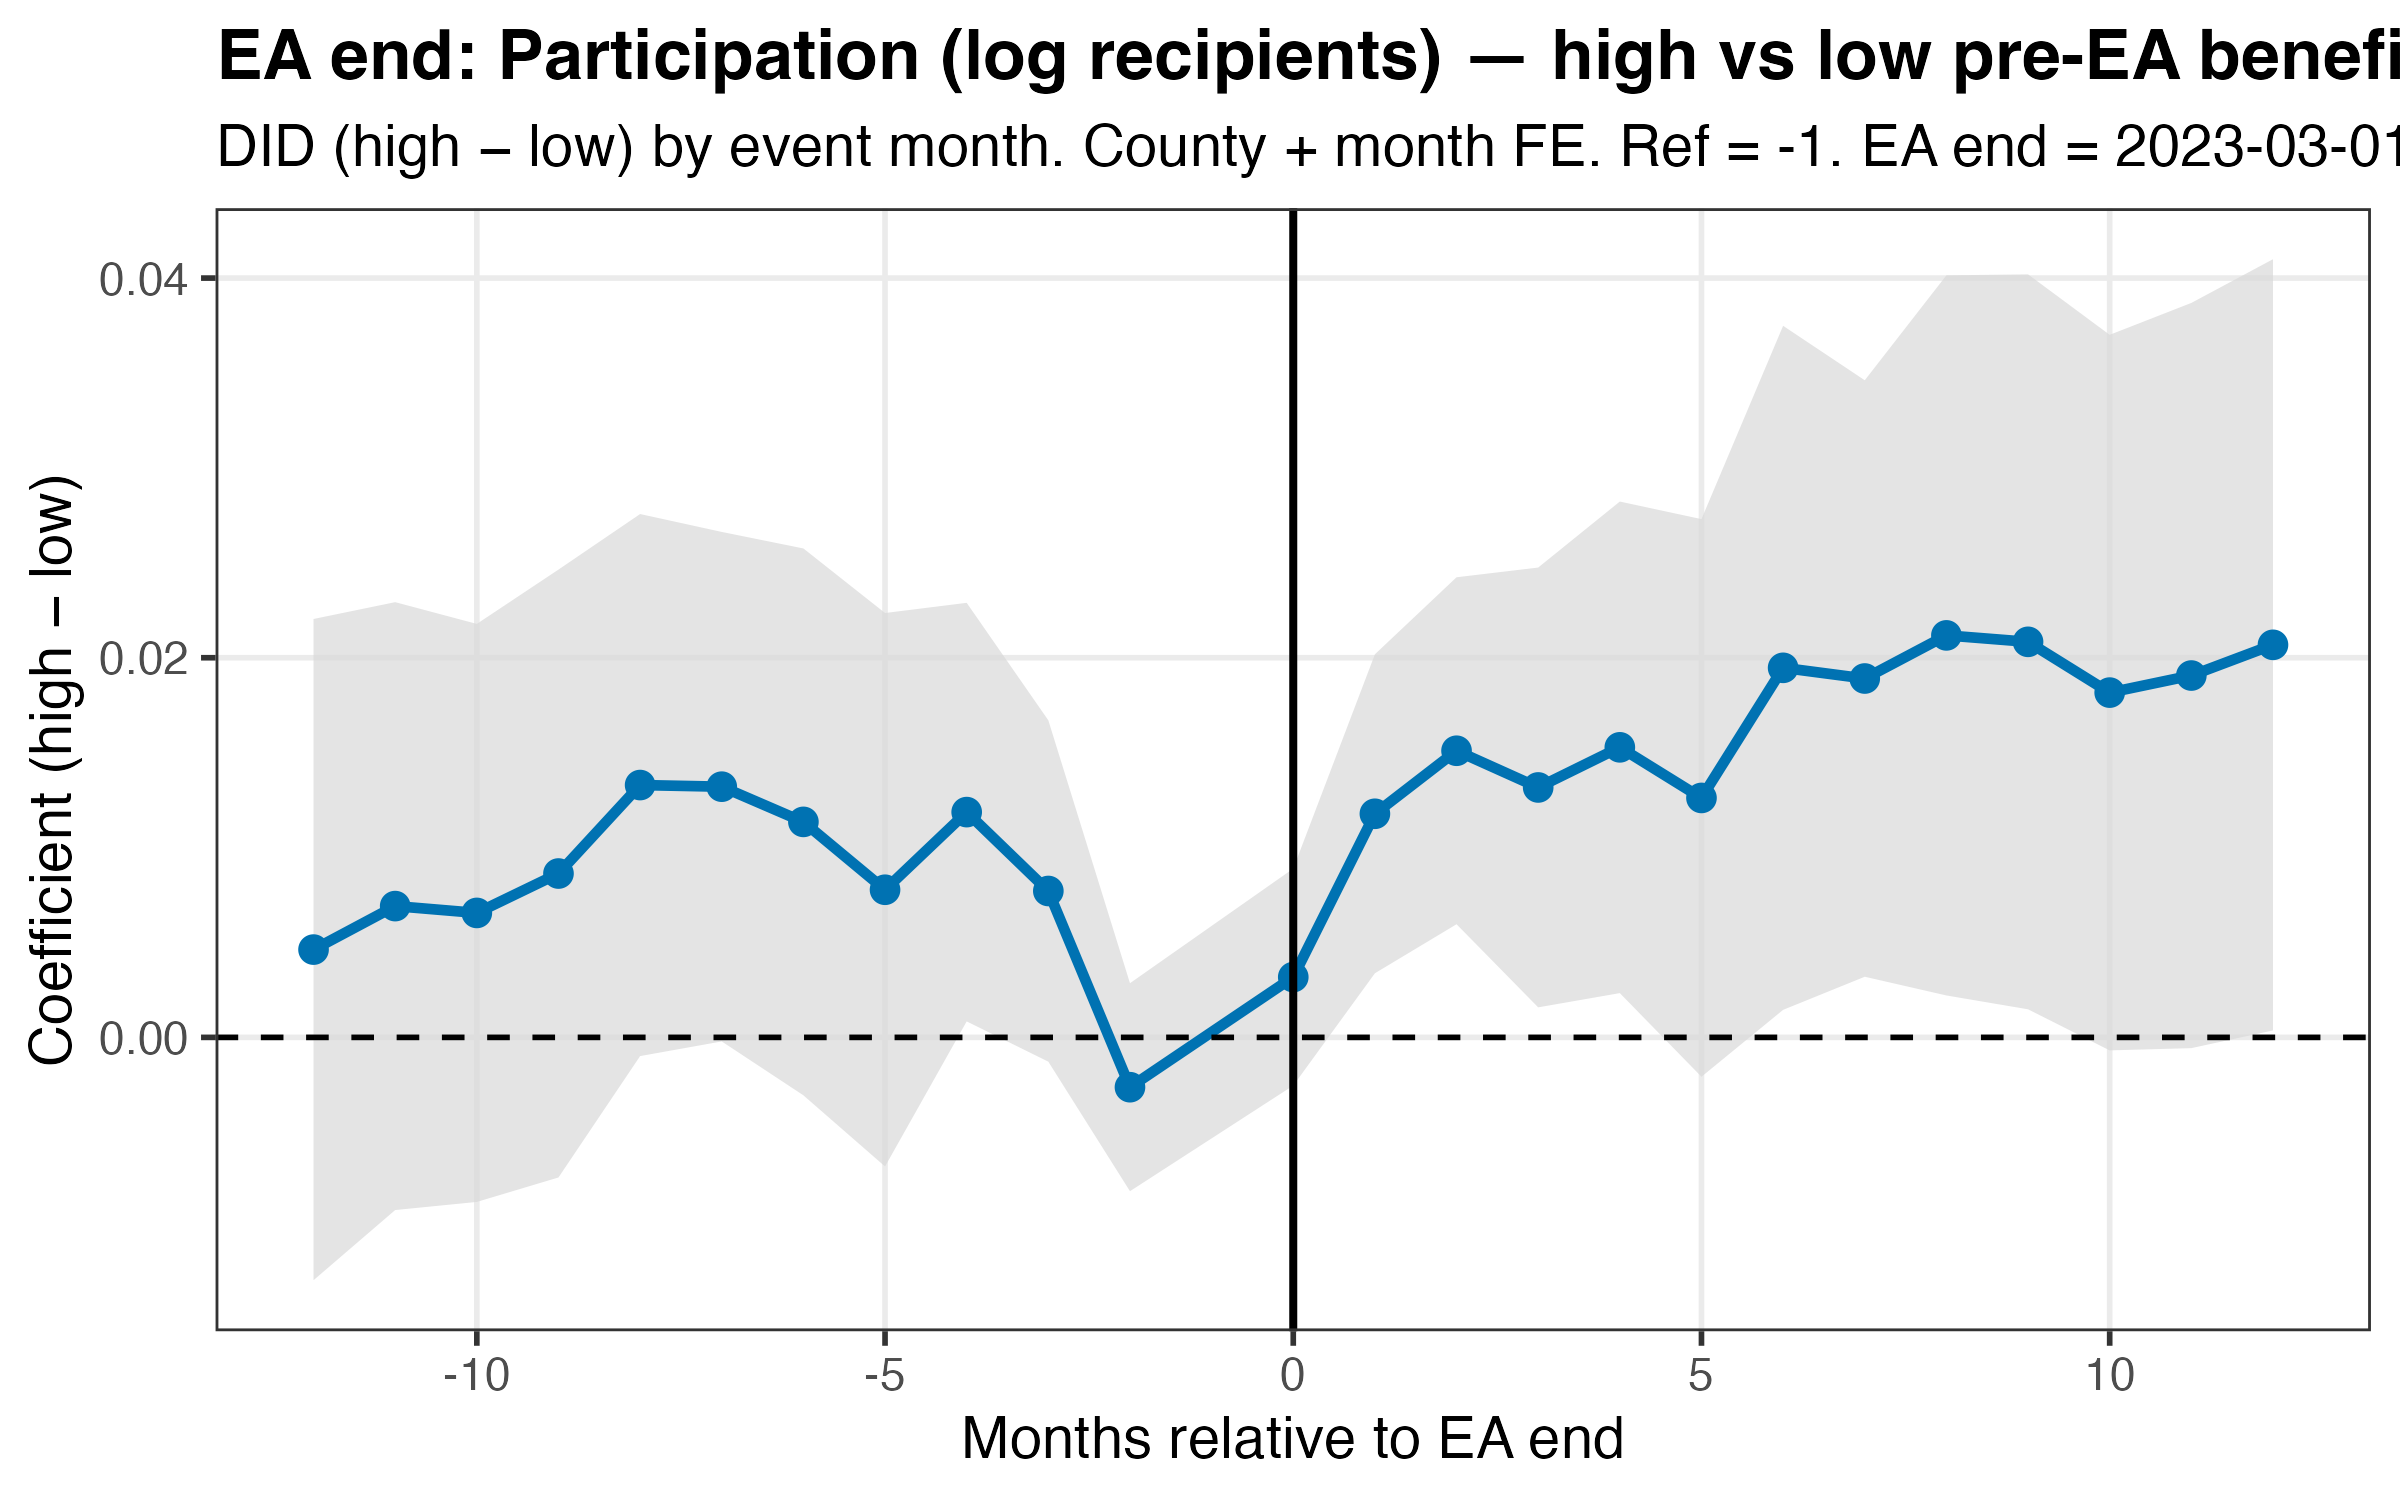
\includegraphics[width=0.85\textwidth]{../outputs/figures/ea_es_participation}
%   \caption{EA end: participation (log recipients), high vs.\ low pre-EA benefit intensity. Differential event-study (high $-$ low); county and month FE; ref.\ month $-1$; 95\% CI; SE clustered by county.}
%   \label{fig:ea-participation}
% \end{figure}

Appendix Table~\ref{tab:ea-heterogeneity-app} reports pre/post mean outcomes by intensity group (descriptive).
